%%
%% This is file `kaumasterstemplate.tex',
%% generated with the docstrip utility.
%%
%% The original source files were:
%%
%% kauthesis.dtx  (with options: `masterstemplate')
%% 
%% This is a generated file.
%% 
%% Copyright (c) 2011-2014 Stefan Berthold <stefan.berthold@kau.se>
%% 
%% This file is part of the kauthesis bundle.
%% 
%% This work may be distributed and/or modified under the
%% conditions of the LaTeX Project Public License, either version 1.3
%% of this license or (at your option) any later version.
%% The latest version of this license is in
%%   http://www.latex-project.org/lppl.txt
%% and version 1.3 or later is part of all distributions of LaTeX
%% version 2005/12/01 or later.
%% 
%% This work has the LPPL maintenance status `author-maintained'.
%% 
%% The Current Maintainer and author of this work is Stefan Berthold.
%% 
%% This work consists of all files listed in manifest.txt.
%% 
%% kauthesis.dtx
%% Copyright (c) 2011-2015 Stefan Berthold <stefan.berthold@kau.se>

\documentclass{kaumasters} % available class options: garamond
\usepackage[swedish]{babel}
\usepackage[T1]{fontenc}
\usepackage[utf8]{inputenc}
\usepackage{titletoc}
\usepackage{geometry}
\usepackage{booktabs}

\usepackage{float}


\usepackage{amsmath}



\usepackage{listings}
\usepackage{pythonhighlight}
\renewcommand{\lstlistingname}{Kodavsnitt}% Listing -> Algorithm
\renewcommand{\lstlistlistingname}{\lstlistingname s avsnitt}% List of Listings ->  Kod avsnitt



%% break long URLs in references.
\usepackage{url}
\def\UrlBreaks{\do\/\do-}
% list
\usepackage{scrextend}
\addtokomafont{labelinglabel}{\sffamily}

\usepackage{fancyhdr}

\usepackage{graphicx}
\graphicspath{{../figures/background/}}
\usepackage[numbers]{natbib}

% clickable

\renewcommand{\baselinestretch}{1.5} 

\usepackage{tabularx}


\makeatletter
\renewcommand\scriptsize{\@setfontsize\scriptsize{7}{8}}
\renewcommand\tiny{\@setfontsize\tiny{5}{6}}
\renewcommand\small{\@setfontsize\small{5}{6}}
\renewcommand\normalsize{\@setfontsize\normalsize{12}{12}}
\renewcommand\large{\@setfontsize\large{10.95}{15}}
\renewcommand\Large{\@setfontsize\Large{12}{16}}
\renewcommand\LARGE{\@setfontsize\LARGE{14.4}{18}}
\renewcommand\huge{\@setfontsize\huge{20.74}{30}}
\renewcommand\Huge{\@setfontsize\Huge{24}{36}}
\makeatother
\usepackage{sectsty}

\chapterfont{\Huge}
\sectionfont{\huge}
\subsectionfont{\LARGE}
\subsubsectionfont{\Large}
\paragraphfont{\Large}


%\pagestyle{fancy}
%\fancyhf{}
%\lhead[\texttit{}]{}
%\rhead[]{}
%\setlength{\headheight}{15pt}

\title{Twitter Sentiment Analysis}
\author{Johan Selberg, Johannes Bandgren}
\supervisor{Kerstin Andersson}
\opponent{Sample Name, Test Fun}
\examiner{Exam}
\institute{Department of Computer Science}
\place{Karlstad Universitet}
\begin{document}

\maketitle


\frontmatter
\begin{abstract}
  Abstract.
  \keywords keywords
\end{abstract}
\approvalpage%
\begin{acknowledgements}
  Thanks.
\end{acknowledgements}

\tableofcontents{}
\listoffigures
\listoftables

\mainmatter
% för att fucka med marginaler
%\newgeometry{top=20mm, bottom=20mm, right=30mm, left=30mm}
\pagestyle{fancy}
\fancyhead[LE,RO]{\thepage}
\fancyhead[RE,LO]{\rightmark}
\fancyfoot{}
\chapter{Introduktion}

\newpage


\chapter{Bakgrund}
Syftet med studien är att utvärdera tre stycken klassificeringsmodeller inom maskininlärning och hur bearbetningen samt märkningen av en datamängd påverkar en klassificeringsmodells prestanda. Maskininlärningsalgoritmerna som kommer att användas för att få fram klassiciferingsmodellerna är Naive Bayes (NB) och Support Vector Machine  (SVM). Den tredje klassificeringsmodellen som tas fram kommer att vara en djuplärande modell  som representeras av ett neuronnät, mer specifikt ett Convolutional neural network (CNN). Figur \ref{fig:overfig} visar en förenklad bild av hur processen för att utvärdera klassificeringsmodellerna kommer att se ut. Datamängden består av en mängd indata som är märkt med förväntad utdata, som går igenom en bearbetningsprocess där t.ex. data som inte tillför något värde tas bort och där mängden av data delas upp i tränings- och valideringsdata.  Bearbetningsprocessen diskuteras mer ingående i \ref{exp:pre}. På den bearbetade datan utförs ett särdragsurval, där dataspecifika särdrag plockas ut…MER .. som diskuteras vidare i \ref{exp:feat}. Träningsmängden används av maskininlärningsalgoritmen för att skapa klassiciferingsmodellen. När klassificeringsmodellen är framtagen används valideringmängden för att utvärdera prestandan av modellen.

\begin{figure}[h]
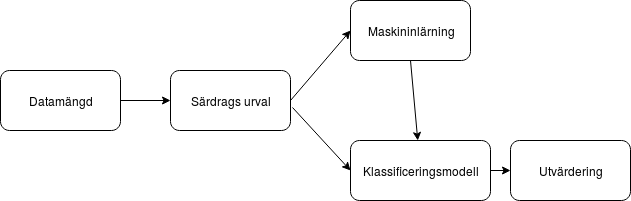
\includegraphics[width=12cm]{oversiktsfigur}
\centering
\caption{Utvärderingsprocessen av maskininlärningsmodeller}
\label{fig:overfig}
\end{figure}

Studien kommer att använda maskininlärning för att utföra sentimentanalys (SA) d.v.s utläsa huruvida en text uttrycker någonting positivt eller negativt. Uppdragsgivaren, CGI, betraktar sentimentanalys  som en viktig pusselbit för framtida lösningar man vill erbjuda sina kunder. Lösningar skulle kunna vara chatbotar där sentimentanalys används så att chatboten ändrar sitt språk utefter svaren från slutanvändare. Eller att det kan användas för trendanalys där ett företag vill veta vad allmänheten tycker före och efter att man har släppt en ny produkt eller efter att kvartalsrapporten har släppts.

I avsnitt \ref{SA} förklaras vad SA är och olika klassificeringstekniker inom SA berskrivs kortfattat. I avsnitt \ref{ML} ges en kort introduktion till maskininlärning och framstegen som gjorts under den senaste tiden. Dessutom beskrivs NB och SVM samt hur inlärningsprocessen ser ut. I avsnitt \ref{DS} ges en överblick över hur en datamängd ser ut och vilka märkningsmetoder som används för twittersentimentanalys (TSA). Avsnittet beskriver även de valda datamängderna. I avsnitt \ref{TSA} ges en introduktion till TSA och vilka utmaning samt problem TSA har. Slutligen i avsnitt \ref{TSAev} förklaras vilka hjälpmedel som kommer att användas för att utvärdera algoritmernas prestanda.


\section{Sentimentanalys} \label{SA}
SA används för att studera människors åsikter, attityder och känslor mot olika entiteter. En entitet kan vara ett ämne, en händelse eller en individ. Målet med SA är att identifiera känslan som är uttryckt i en text för att därefter analysera den. Processen delas upp i tre steg: att hitta entiteter, identifiera känslan för de entiteterna och slutligen klassificera dessa entiteter. \cite{SAsurvey}.

Inom SA appliceras klassificeringen på 3 olika nivåer: dokument-, menings- och aspektnivå \cite{SAsurvey}. SA på dokumentnivå klassificerar om ett helt dokument uttrycker en positiv eller negativ åsikt, exempel på dokument kan vara produktrecensioner eller nyhetsartiklar. Medan på meningsnivå klassificeras varje mening i ett dokument. Slutligen nere på aspektnivå analyseras de möjliga aspekterna av en entitet. En mening kan behandla olika aspekter av en entitet. Både positiva och negativa åsikter kan delges om en entitets olika aspekter. Ett exempel på det är meningen “Ölen var väldigt god, men tyvärr alldeles för dyr”, som innehåller både en positiv och en negativ åsikt om en entitet som i det här fallet är ölen.
\subsection{Klassificeringstekniker} \label{SAkt}
De olika klassificeringsteknikerna som i nuläget används för SA delas upp i 3 olika kategorier: maskininlärningsmetoder, lexikonbaserade metoder samt hybrida metoder \cite{SAsurvey}. 

Maskininlärningsmetoder använder etablerade maskininlärningsalgoritmer tillsammans med språkliga särdrag för att konstruera klassificerare som kan avgöra om en text uttrycker någonting positivt eller negativt [ref=Sentiment analysis a survey]. Prestandan för maskininlärningsmetoder är beroende av mängden träningsdata, större mängder data ger vanligtvis bättre resultat \cite{TSAsurvey}. Maskininlärningsmetoder är dessutom domänberoende, vilket gör att de inte presterar bra när de används på andra domäner än det de har tränats på. 

Lexikonbaserade metoder använder sig av ordlistor för att analysera text \cite{SAsurvey}. Ordlistorna består av positiva och negativa termer som används för att beräkna vad en given text uttrycker för sentiment.
Fördelen med lexikonbaserade metoder är att de inte kräver någon  träningsdata \cite{TSAsurvey}. Men faktumet att de är beroende av statiska ordlistor betyder att de inte tar hänsyn till termer som inte finns i ordlistorna. Det betyder att ordlistor måste uppdateras kontinuerligt för innehåll som är dynamiskt och ständigt under utveckling, vilket är särskilt problematiskt för texter som förekommer på sociala medier. 

Hybrida metoder kombinerar lexikonbaserade metoder med maskininlärningsmetoder \cite{TSAsurvey}. Genom att kombinera metoderna med varandra kan de väga upp för varandras svagheter. Nackdelen med hybrida metoder är dock att de kräver en hög beräkningskomplexitet.

Experimentet som presenteras i studien fokuserar enbart på maskininlärningsmetoder.

\section{Maskininlärning} \label{ML}
Maskininlärning är ett delområde inom artificiell intelligens (AI), där målet är att göra det möjligt för datorer att lära sig på egen hand. Maskininlärningsalgoritmer gör det möjligt att identifiera olika mönster från observerad data, bygga upp en generell modell som kan förutsäga saker utan att ha blivit förprogrammerade med explicita regler för hur den ska lösa ett problem. Under de senaste åren har stora framsteg inom maskininlärning gjorts. Exempelvis utvecklade DeepMind \cite{DMatari00} 2015 en agent som mästrade 49 st Atari-spel \cite{wiki:004}, med en klassificeringsmodell med endast pixlar och spelpoäng som indata. Under 2016 utvecklade DeepMind sin AlphaGo \cite{DMgo} agent som besegrade en av världens bästa Go spelare, Lee Sedol \cite{wiki:005} med 4-1 i matcher. Detta var ett framsteg för AI eftersom Go är ett komplext spel med $2 * 10^{170}$ möjliga drag \cite{wiki:006}.

Maskininlärning används också för att lösa vardagliga problem. I dagens mobiltelefoner finns en så kallad intelligent personlig assistent, även kallade Siri \cite{siri} och Google Assist \cite{google},  där användarna får hjälp med t.ex. “vad är det för väder idag?”, “Skicka ett meddelande till mamma att jag blir sen till middagen idag” och “Påminn mig imorgon att jag måste köpa mjölk”. Facebook använder även maskininlärning för ansiktsigenkänning \cite{facebook:001} på bilder som laddas upp, och för att rekommendera nya vänner \cite{facebook:002}. 

%\section{Övervakad och oövervakad inlärning} \label{MLvised}
Figur \ref{fig:ml} illustrerar att maskininlärning delas upp i två typer av inlärningsprocesser dvs. i övervakad eller oövervakad inlärning och deras underliggande algoritmer.
\begin{figure}[h]
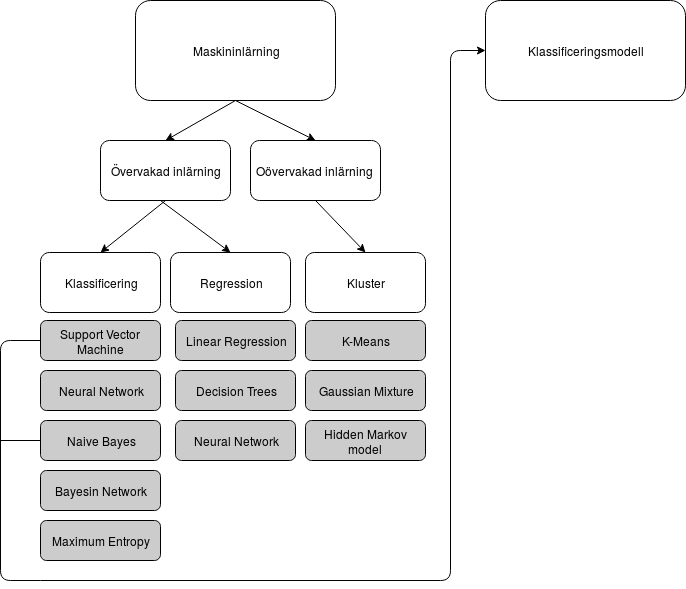
\includegraphics[width=12cm]{ml}
\centering
\caption{Inlärningsprocesser för maskininlärning.}
\label{fig:ml}
\end{figure}

Oövervakad inlärning används när datamängden bara består av indata och inget förväntat resultat. Målet med oövervakad inlärning är att algoritmen själv lär sig att modellera den komplexa underliggande strukturen så att den kan lära sig mer om datan och själv komma fram till ett resultat \cite{wiki:007}. Exempelvis kan en oövervakad klusteralgoritm användas för att hitta likheter i bilder och följaktligen gruppera dem.
Övervakad inlärning används när datamängden består av både indata och dess förväntade utdata. Den övervakade algoritmen använder datamängden för att lära sig hur utdata beror på indata genom att skapa en klassificeringsmodell som används för att förutse utdata från ny indata som illustreras i figur \ref{fig:kl}. 

Övervakad inlärning kan man tänka sig som att en lärare övervakar programmets inlärningsprocess. Under inlärningsprocessen försöker algoritmen iterativt förutse utdata från datamängden och blir rättad av läraren vid fel förutsägelse \cite{learning:001}.

\begin{figure}[h]
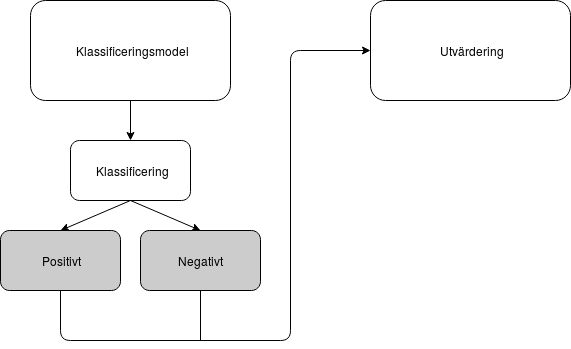
\includegraphics[width=12cm]{klassmodell}
\centering
\caption{Klassificeringsprocess av data.}
\label{fig:kl}
\end{figure}

Övervakad inlärning kan brytas ner till klassificerings- och regressionsproblem och eftersom TSA kan kallas ett typiskt klassificeringsproblem \cite{SAsurvey}, kommer studien att använda algoritmer lämpade för klassificeringsproblem. I figur \ref{fig:ml} kan vi se några av dessa klassificeringsalgoritmer och enligt \cite{TSAsurvey} är speciellt Naive Bayes (NB) och Support Vector Machine (SVM)  bäst lämpade för TSA.

\subsection{Naive Bayes} \label{MLnb}
NB är en klassificeringsalgoritm som är baserad på Bayes theorem \cite{wiki:009} med starka (“naive”) oberoende antaganden mellan särdragen d.v.s NB förutsätter att närvaron av ett visst särdrag i en klass inte relaterar till närvaron av ett annat särdrag. 
Exempelvis kan en frukt anses vara ett äpple om det är grönt, runt och är 10 cm i diameter. Även om särdragen grönt, runt och diameter kan bero på varandra så bidrar alla särdragen självständigt till sannolikheten att frukten är ett äpple, det är därför algoritmen kallas (“naive”) \cite{nb:001}.

\subsection{Support Vector Machine} \label{MLsvm}
SVM är en övervakad maskininlärningsalgoritm som kan användas till både klassificerings- och regressionsproblem, för det mesta används SVM för klassifikationsproblem. SVM är baserat på idén att hitta ett hyperplan \cite{svm:001} som bäst delar upp datamängden i två klasser \cite{svm:003}. Givet en träningsmängd där förväntad utdata är markerad till en av två kategorier bygger SVM-algoritmen upp en klassificeringsmodell som kan användas för att förutse vilken kategori ny indata ger \cite{svm:002}. 

\subsection{Convolutional neural network}\label{bak:cnn}
Ett av de snabbast växande områden inom maskininlärning är djup inlärning \cite{TSAsurvey}. Begreppet djup inlärning syftar till artificiella neuronnät (ANN) som är uppbyggda med flera lager  \cite{cnn:001}. ANN är system som försöker ta efter beteende hos biologiska neuronnät för att stegvis bli bättre på att utföra en angiven uppgift genom att studera exempel \cite{wiki:015}. 

CNN är ett av de mest populära neuronnäten  \cite{cnn:001}. Det var ursprungligen framtaget för maskininlärningsproblem som rör datorseende och har tidigare påvisat imponerande resultat för bildigenkänning \cite{cnn:003, cnn:006}. Men på senare tid har det även visat sig att CNN är effektivt att använda för problem som rör sentimentanalys. Med relativt enkla CNN-modeller har imponerande resultat kunnat uppnås inom textklassificering.  I \cite{cnn:003} presenteras en enkel CNN-modell för textklassificering som påvisade goda resultat över flertalet datamängder. CNN-modellen som har använts i den här studien har utgått från den modell som Yoon Kim presenterar i \cite{cnn:003}.

\section{Datamängd} \label{DS}
En datamängd för övervakad inlärning består av en mängd in- och utdata som diskuteras i sektion \ref{ML}. Processen för hur rätt utdata (positiv/negativ) märks kan utföras på två olika sätt, antingen genom så kallad mänsklig märkning där människor markerar indata som positiv/negativ eller genom “distant supervision” där en dator märker indata som positiv/negativ utefter någon parameter. Den stora skillnaden mellan mänsklig märkning och “distant supervision” är att “distant supervision” kan generera en mycket större datamängd än mänsklig märkning men risken är större att märkningen blir felaktig \cite{TSAsurvey}. 
Som är beskrivit i sektion \ref{bac:intro} är ett delsytfte med denna studie att utvärdera hur de olika märkningsmodellerna påverkar maskininlärningsalgoritmernas precision. Det finns ett urval med publika twitterdatamängder där både mänsklig märkning och “distant supervison” används \cite{TSAsurvey}. Vi har valt att använda datamängderna Stanford Twitter Sentiment (STS) \cite{sts:001} och SemEval \cite{SemEval:001} eftersom de är de största publika datamängderna inom respektive märkningsmodell.

\subsection{SemEval} \label{DSse}
SemEval-datamängden består av 20633 tweets och är framtagen till en årlig TSA-tävling som har gått sedan 2013 \cite{SemEval:002}. 
För datamängden har mänsklig märkning tillämpats, där fem personer manuellt märker varje tweet via Amazon Mechanical Turk \cite{SemEval:003}.
I \cite{SemEval:004} beskrivs metoden för hur märkningen utförs, varje person markerar varje tweet antingen som mycket positivt, positivt, neutralt, negativt eller mycket negativt. Efter att alla tweets är märkta kartläggs alla tweets till kategorierna positivt, neutralt eller negativt utefter tre kriterier. Antingen att alla personer har märkt en tweet samma, en majoritet har märkt samma eller genom att ta ut ett medelvärde. Medelvärdet räknas ut genom att kartlägga de fem kategorierna till heltal mellan 2 och -2, medelvärdet räknas sedan ut och kartläggs till den närmsta kategorin. För SemEval-datamängden blev utfallet 2760 tweets där alla personer gjort samma märkning, 9944 tweets är där majoritet har märkt samma och för resterande 7928 tweets har medelvärdet räknats ut. 

\subsection{Stanford Twitter Sentiment} \label{DSsts}
STS-datamängden är framtagen mellan April 2009 och Juni 2009 av Alec Go, Richa Bhayani och Lei Huang. STS-datamängden är märkt med hjälp av “distant supervision” där märkningen bestäms av vilken typ av emoji \cite{wiki:010} ett twitterinlägg innehåller, exempelvis märks ett twitterinlägg positivt om det innehåller “:), :-),: ), :D, =)” och negativt om det innehåller “:(, :-(, : (“ \cite{sts:001}. 

\section{Twittersentimentanalys} \label{TSA}
TSA är den del av SA som specifikt handlar om att analysera inlägg som användare gör på Twitter. Twitter är en av de populäraste mikrobloggarna där användare kan skriva och kommunicera med varandra genom twitterinlägg. 2013 var Twitter en av de tio mest besökta sidorna på internet och 2016 uppmättes antalet aktiva användare per månad till 319 miljoner. Twitter är definierat som en mikroblogg på grund av det låga antalet tecken som är tillåtet för ett inlägg. I November 2017 fördubblades antalet tillåtna tecken från de tidigare 140 till 280 \cite{wiki:008}. 

Det finns en rad olika begrepp som kännetecknar Twitter och som är viktiga att känna till \cite{TSAsurvey}. En “tweet” är vad som tidigare nämnts ett twitterinlägg. Det är ett inlägg från en användare som är begränsat till 280 tecken, där användaren exempelvis kan delge sina åsikter i olika ämnen eller dela med sig av personliga upplevelser. En “tweet” behöver inte enbart innehålla ren text utan kan även innehålla länkar, bilder och videor. I fortsättningen av rapporten kommer en “tweet” att benämnas twitterinlägg.

När ett twitterinlägg innehåller “mentions” betyder det att andra användare nämns i inlägget. Det kan vara användbart för att exempelvis delge åsikter om andra användare eller för att öppet starta en diskussion med en nämnd användare. För att nämna en användare i ett twitterinlägg skrivs symbolen @ före användarnamnet. 

På Twitter har användare möjligheten att följa andra användare. Det betyder att användare kan följa andra användares aktivitet i deras egna twitterflöden och dela med sig av sin egen aktivitet till sina följares twitterflöden. En användare som följer en annan benämns på Twitter som en “follower”. Att följa andra är det primära tillvägagångssättet för att skapa kontakter med andra användare på Twitter. 

Användare har möjlighet att kategorisera twitterinlägg och det är vad “hashtags” används för. Genom att använda “hashtags” kan användare märka sina twitterinlägg med etiketter för att knyta inlägget till ett specifikt ämne. Användandet av hashtags gör det enkelt för användare att följa ett ämne. De behöver enbart söka på en specifik “hashtag” för att få fram alla twitterinlägg i ämnet. För att skapa en “hashtag” skrivs symbolen \# före namnet på etiketten.

Det är även möjligt att dela andra användares twitterinlägg till ens egna följare. Den funktionen kallas för “retweet” och ett sådant twitterinlägg startar vanligtvis med förkortningen RT följt av en “mention” av den ursprungliga författaren av twitterinlägget. Det kan exempelvis vara användbart för att sprida information till följare eller för att skapa en diskussion om innehållet i twitterinlägget med sina egna följare. 

När användare svarar på andras twitterinlägg benämns det som “replies” och det är till för att det ska gå att skapa konversationer, där det ska gå att urskilja vanliga twitterinlägg från svar på twitterinlägg. En användare svarar på ett twitterinlägg genom att göra en referens till den ursprungliga författaren av inlägget följt av svaret på inlägget.

Användare behöver inte göra alla sina inlägg offentliga för alla användare, de kan begränsa synligheten för deras twitterinlägg att enbart synas för deras egna följare. 

I figur \ref{fig:tweet} presenteras ett exempel på hur ett twitterinlägg kan se ut. Twitterinlägget är en “retweet som ursprungligen har skrivits av användaren johanselberg. Det innehåller en “hashtag” med etiketten exempel och en “mention” av användaren KAU. Twitterinlägget innehåller även en extern länk.

\begin{figure}[h]

\includegraphics[width=12cm]{exempeltweet}
\centering
\caption{Twitterinlägg innehållande ''hashtag'', ''mention'', ''retweet''.}
\label{fig:tweet}
\end{figure}

\subsection{Utmaningar} \label{TSAchall}
På grund av restriktionen av antalet tillåtna tecken i ett twitterinlägg innehåller majoriteten av twitterinlägg enbart en mening. Därför är det skillnad på klassificeringsnivåerna i TSA och SA. I TSA är det ingen skillnad på dokument- och meningsnivå. Därför används det enbart två klassificeringsnivåer inom TSA: meningsnivå (meddelandenivå) och aspektnivå. \cite{TSAsurvey}

Restriktionen av antalet tillåtna tecken utgör den stora skillnaden mellan TSA och SA. Att analysera sentiment på en text i ett twitterinlägg skiljer sig markant från att göra det på vanliga texter som återfinns i produktrecensioner och nyhetsartiklar. Det gör att TSA ställs inför en rad andra utmaningar än vad SA ställs inför.

I \cite{TSAsurvey} tar författarna upp de viktigaste utmaningar med TSA. För att bra resultat ska uppnås med TSA måste dessa utmaningar hanteras. Det som ligger till grund för utmaningarna med TSA är huvudsakligen restriktionen av antalet tillåtna tecken, att det är en informell typ av medium samt att innehållet på Twitter är dynamiskt och ständigt utvecklas.

Det låga antalet tillåtna tecken och att det är en informell typ av medium, gör att språket som används på Twitter skiljer sig från språket som används i vanlig text. Twitterinlägg innehåller ofta felaktigt språkbruk. Det är vanligt förekommande att Twitterinlägg innehåller förkortningar, slang,  nybildade ord och att ord betonas genom att de förlängs eller att de skrivs med versaler. 

På grund av att användandet av felaktigt språkbruk är så pass vanligt på Twitter, innehåller twitterinlägg en hel del brus. Felstavade termer gör att antalet gånger en specifik term förekommer i en mängd av text blir mindre. Det resulterar i datagleshet (data sparsity) och har en negativ påverkan på resultatet vid SA. För att minska dataglesheten omvandlas vanligtvis felstavade termer till den korrekta stavningen eller en mer korrekt stavning.

En annan utmaning med TSA är att hantera negationer, vilket även gäller SA. Om negationer förekommer i ett twitterinlägg kan det vända på inläggets sentiment. Därför är det viktigt att kunna tolka och identifiera negationer för att sentimentanalysen ska bli korrekt.

I många fall av SA analyseras texter som är skrivna på ett specifikt språk, exempelvis när nyhetsartiklar utgivna av en viss tidning analyseras. Vid TSA är det inte lika enkelt eftersom twitterinlägg kan vara skrivna på flera olika språk och det är inte ovanligt att språk blandas i inlägg. Den här studien kommer enbart analysera twitterinlägg skrivna på engelska och inhämtade inlägg skrivna på annat språk kommer filtreras bort. 

Vid TSA filtreras vanligtvis stoppord bort för att öka prestandan. Stoppord är ord som är vanligt förekommande i texter men som saknar någon större betydelse för texten ifråga. I engelskan är “the”, “is” och “who” exempel på stoppord.

Twitterinlägg behöver inte enbart innehålla text utan de kan även innehålla bilder och videor. Bilder och videor kan ge värdefull information om vad för sentiment som uttrycks i ett twitterinlägg. Det kan exempelvis ge information om vem som uttrycker en åsikt eller om vem en åsikt riktas mot. Den här studien kommer inte att ta hänsyn till mediaobjekt utan kommer enbart att analysera text. Främst på grund av att det i dagsläget är ett outforskat område.

\subsection{Problem} \label{TSAprob}
I \cite{TSAsurvey} listar författarna de problem med TSA som de anser bör utforskas ytterligare. Ett av de viktigaste problemen med TSA anser de vara bristen på datamängder som kan användas som riktmärken vid utvärdering av olika klassificeringsmodeller. Forskning som bedrivs i ämnet använder sig av olika datamängder. Dessutom är det vanligt att forskare själva samlar in och skapar egna datamängder som inte publiceras. Olika datamängder kan generera olika resultat. Därför är det svårt att jämföra olika klassificeringstekniker när det används flertalet olika datamängder. I experimentet, som presenteras i den här studien, har problemet adresserats genom att utvärderingen görs mot två kända och publika datamängder. Delvis för att kunna jämföra hur de olika klassificeringsmodellerna presterar mot olika typer av datamängder, men även för att kunna jämföra resultatet mot andra liknande utvärderingar.
\begin{table}
\centering
\caption{Förvirringsmatris}
\label{tab:fm}
	\begin{tabular}{ccc}
	\toprule
	 & \textbf{Förustspådd positiv} & \textbf{Förutspådd negativ} \\
	\midrule
	\textbf{Positiv} & Sann positiv & Falsk negativ \\
	\textbf{Negativ} & Falsk positv & Sann negativ \\
	\bottomrule
\end{tabular}
\end{table}

\section{Utvärdering} \label{TSAev}
I tabell \ref{tab:fm} ser vi en så kallad förvirringsmatris (FM) som utvärderar en klassificeringsmodell från datamängden där “positivt” eller “negativt” är förbestämt. Matrisen visar antalet sann positiv (SP), sann negativ (SN), falsk positiv (FP) och falsk negativ(FN) \cite{wiki:003}. Med dessa värden kan vi jämföra och analysera modellerna m.h.a följande utvärderingsmetoder: noggrannhet (n) \cite{wiki:011}, precision (p),  återkallelse (å) \cite{wiki:002} och F-Score \cite{wiki:001}.

\begin{labeling}{metrics}
\item [Noggrannhet] Är modellens förmåga att kunna märka ett twitterinlägg korrekt som antingen positivt eller negativt. Detta görs genom att ta summan av sannmärkta tweets delat på summan av alla märkningar.  
\item [Precision]  Är förmågan att modellen inte märker ett tweet som positivt när det är negativt. Detta görs genom att ta antalet sann positiva delat på totalt antal positivt märkta tweets. 
\item [Återkallelse] Är förmågan att modellen märker positiva tweets korrekt. Detta görs genom att ta antalet sann positiva delat på summan av antalet sann positiva och falsk negativa.
\item [F-Score] Även kallat det harmoniska medelvärdet mellan precision och återkallelse används då inte alltid precision och återkallelse räcker till för att göra en helhetsbedömning. 
\end{labeling}

I figur \ref{fig:utv} illustreras hur utvärderingmetoderna hänger ihop.

\begin{figure}[h]
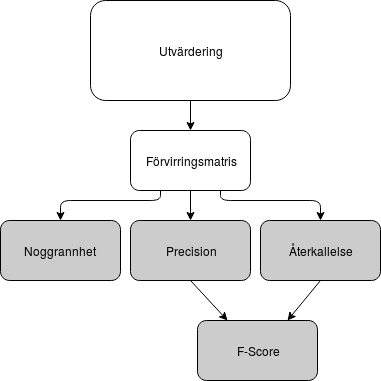
\includegraphics[width=10cm]{utvardering}
\centering
\caption{Utvärderingsmetoder för TSA.}
\label{fig:utv}
\end{figure}


\section{Sammanfattning} \label{BACKsum}
I detta kapitel har bakgrunden till projektet diskuterats och där nyttan av SA och TSA har tagits upp. Intressant för uppdragsgivaren är hur de kan integrera SA och TSA i sina produkter t.ex. chatbotar och trendanalys. 

Detta kapitel ger även en överblick av vad maskininlärning är och hur maskininlärningens viktigaste komponenter hänger ihop samt hur maskininlärning kan appliceras på SA och TSA. Dessutom beskrivs de problem och utmaningar som existerar inom TSA. 

\chapter{Experiment}
I kapitlet kommer experimentet för studien att presenteras, hur det har utförts och hur de olika delarna har implementeras. Delarna utgörs av bearbetning av datamängderna, vilka särdragsurval som kommer utföras och en fördjupning i hur maskininlärningsalgoritmerna fungerar. Implementationen kommer ske i tre steg där först en lexikonbaserad modell kommer tas fram, för att ge ett basfall för respektive datamängd, för att sedan implementera algoritmerna med standardparametrar och slutligen testa och justera algoritmernas parametrar. Detta för att eventuellt uppnå en högre precision för respektive klassificeringsmodell. 
De slutgiltliga klassificeringsmodellerna kommer att diskuteras och jämföras i avsnitt \ref{res}.
\section{Bearbetning av datamängd} \label{exp:pre}
En viktig del inom SA är bearbetningen av den data som ska analyseras. Bearbetning av data, i fallet SA, handlar om att tvätta och förbereda texter som ska klassificeras \cite{effrosynidis2017comparison}. 

Kvaliteten på data som ska analyseras är avgörande för vilka resultat som kan uppnås vid maskininlärningen \cite{effrosynidis2017comparison}. I \cite{HADDI201326} rapporteras att bearbetning av text innan maskininlärning kan ha en tydlig positiv påverkan på en klassificeringsmodells prestanda vid sentimentanalays. Därför behöver data som ska analyseras bearbetas innan maskininlärningen, vilket betyder att data normaliseras och reduceras på brus. Teorin med att bearbeta en datamängd innan maskininlärningen är att det delvis kan förbättra prestandan för klassificeringsmodellen men även att  klassificering kan utföras snabbare, vilket kan vara av betydelse för sentimentanalys som utförs i realtid \cite{7862202}. 

Som nämndes i avsnitt \ref{TSAchall}, innehåller twitterinlägg vanligtvis stora mängder brus på grund av det informella språket som används på Twitter, dvs data som inte är användbar för analysprocessen. Det finns exempelvis många ord som inte har någon påverkan på en texts sentiment och därför är det vanligtvis inte nödvändigt att ta med alla ord från den ursprungliga texten vid maskininlärning \cite{effrosynidis2017comparison, HADDI201326}. Ord som dessa kan tas bort, ersättas eller slås samman med andra. Det är det som kallas för att bearbeta data. Genom att göra det minskas dimensionen på problemet och textklassificeringen blir enklare att utföra , eftersom varje ord behandlas som en dimension \cite{HADDI201326}. 

Det existerar flertalet olika tekniker som kan användas vid bearbetningen av data, vissa mer vanliga än andra. I arbetet med studien har två artiklar använts som undersöker effekten av olika bearbetningstekniker vid TSA, \cite{effrosynidis2017comparison} och \cite{7862202}. Båda artiklarna utvärderar bearbetningsteknikerna utefter hur de påverkar prestandan vid sentimentklassificering.

I \cite{effrosynidis2017comparison} utvärderas 15 olika bearbetningstekniker. Teknikerna utvärderas var för sig och testas mot två olika datamängder, där de för varje datamängd testas med tre olika klassificeringsmodeller.  Några bearbetningstekniker ger bättre noggrannhet för båda datamängderna, andra sämre och resultaten varierar för några. Resultaten varierar inte enbart mellan datamängderna utan de varierar även mellan klassificeringsmodellerna. De tekniker som rekommenderas av författarna och resulterar i hög noggrannhet för alla klassificeringsmodeller och de båda datamängderna är: borttagning av nummer, omvandling av ord till deras ursprungliga form samt ersättning av upprepade skiljetecken. Hantering av negationer, lemmatisering samt ersättning av URL:er och “mentions” av användare påvisar också bra resultat för båda datamängderna men dock inte för alla klassificeringsmodeller. Borttagning av skiljetecken var den bearbetningsteknik som gav sämst resultat. Det som saknas i \cite{effrosynidis2017comparison} är hur de olika förbehandlingsteknikerna presterar i kombination med varandra, vilket enligt författarna själva kan ge andra resultat.

Detta är dock något som görs i \cite{7862202}. Istället för att utvärdera teknikerna isolerade från varandra som i \cite{effrosynidis2017comparison}, utvärderas de istället utifrån hur de presterar i kombination med andra. Dock har de enbart valt att fokusera på sex olika bearbetningstekniker: expandering av sammandragsförkortningar, expandering av förkortningar, avlägsning av nummer, avlägsning av stoppord, ersättning av förlängda ord och avlägsning av URL:er. Bearbetningsteknikerna har utvärderats utefter hur de presterar på fem olika datamängder på fyra klassificeringsmodeller. Vid bedömningen av prestandan vid sentimentklassificeringen har ett basfall använts. Basfallet har använt samtliga sex bearbetningstekniker för bearbetningen av datan vid testningen. När en specifik teknik har utvärderats, har tekniken i fråga exkluderats från mängden av bearbetningstekniker. Därefter har testerna repeterats, med fem bearbetningstekniker istället för sex. Sedan har förändringen av resultatet gentemot basfallet använts för att bedöma hur tekniken påverkar prestandan vid sentimentklassificeringen. Resultaten visar att expandering av sammandragsförkortningar och expandering av förkortningar kan ha positiv påverkan på noggrannheten vid klassificeringen. Avlägsning av URL:er, nummer och stoppord påverkar resultaten för klassificeringen minimalt, men är effektiva för att minska brus. 

Utifrån resultaten som har presenterats i \cite{effrosynidis2017comparison} och \cite{7862202} har bearbetningsteknikerna för experimentet i den här studien valts. 
Det svåra med att välja bearbetningstekniker, utifrån litteraturen, är att det kan existera flera olika varianter av en viss teknik och att olika namn kan användas för att beskriva en viss teknik. I \cite{effrosynidis2017comparison} hanterar de exempelvis URL:er genom att ersätta varje URL med etiketten “URL”, medan de avlägsnas helt i \cite{7862202}. Eftersom bearbetningsteknikerna uteslutande kommer att användas i kombination med varandra vid det här experimentet har störst vikt lagts på de tekniker som presenteras i \cite{7862202}.

\begin{figure}[H]
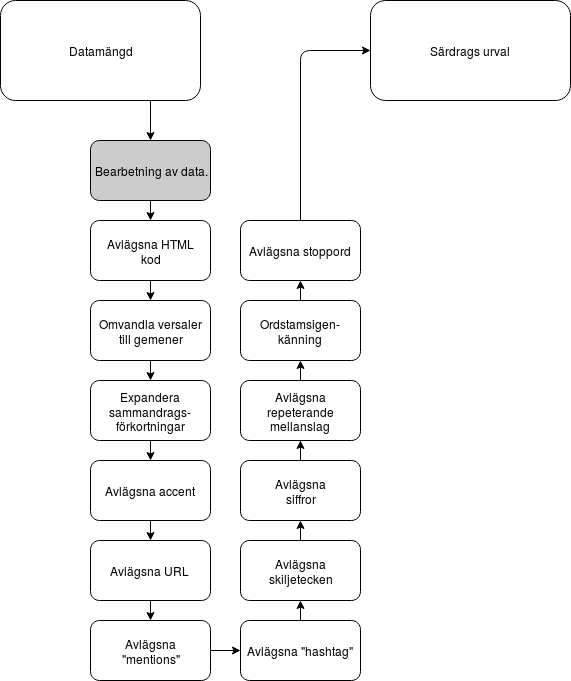
\includegraphics[width=12cm]{dataset}
\centering
\caption{Bearbetningstekniker som används för att bearbeta data vid experimentet.}
\label{fig:dataset}
\end{figure}

Nedan presenteras och beskrivs de bearbetningstekniker som har valts att användas för experimentet. De valda teknikerna visualiseras i figur \ref{fig:dataset}. För några av bearbetningsteknikerna har ordningen betydelse. Exempelvis kommer inte expanderingen av sammandragsförkortningar kunna genomföras ifall avlägsnandet av accenter sker innan. Totalt har 13 bearbetningstekniker använts. Majoriteten av dessa handlar om att avlägsna text från twitterinläggen. Det som avlägsnas vid bearbetningen av twitterinläggen är: HTML-kod, accenter, URL:er, “mentions”, “hashtags”, skiljetecken, siffror, repeterande mellanslag, emojis och stoppord. Avlägsning av emojis diskuteras i avsnitt \ref{exp:feat}. Stoppord, som beskrevs i \ref{TSAchall}, tas bort genom att twitterinläggen söks igenom på stoppord från en fördefinierad lista. Trots att man i \cite{effrosynidis2017comparison} rapporterar sämre prestanda vid avlägsning av skiljetecken har det valts att användas som en bearbetningsteknik för det här experimentet. Det valet gjordes eftersom att man i  \cite{effrosynidis2017comparison} samtidigt rapporterar att det bidrar till att reducera storleken på klassificeringsproblem. 

De övriga teknikerna som används omvandlar text under bearbetningen av ett twitterinlägg. Ett av de första stegen i den bearbetningsprocess, som har använts för detta experiment, är att omvandla versaler i ett twitterinlägg till gemener. Det gör att ord som är skrivna på flera olika sätt slås samman till ett \cite{effrosynidis2017comparison}. Vokabulär blir då mindre, vilket gör att storleken på problemet minskas.

En annan teknik som används är att expandera sammandragsförkortningar.  I \ref{TSAchall} diskuterades vikten av att kunna tolka och identifiera negationer för att SA ska bli korrekt. Eftersom sammandragsförkortningar är vanligt förekommande i engelskan fokuserar tekniken på att expandera sammandragsförkortningar med motsägelser. Exempelvis är termen “don’t” exempel på en sammandragsförkortning för motsägelsen “do not”. För experimentet har sammandragsförkortningarna “n’t”, “can’t” och “won’t” omvandlats till “not”, “can not” och “will not”, utefter hur metoden beskrevs i \cite{7862202}.

Slutligen har också ordstamsigenkänning använts vid bearbetningen av ett twitterinlägg. Ordstamsigenkänning går ut på att ta bort ändelser från ord för att omvandla dem till deras ursprungliga form \cite{effrosynidis2017comparison}. Det leder också till att ord slås samman och att storleken på problemet minskar. Tabell \ref{tab:stemming} visar ett exempel på vad som sker då ordstamsigenkänning används på olika böjningar av det engelska ordet ''arrive''.

\begin{table}[H]
\centering
\caption{Exempel på vad som sker när ordstamsigenkänning används på olika böjningar av det engelska ordet ''arrive''.}
\label{tab:stemming}
    \begin{tabular}{cc}
 	\toprule
    \textbf{Före} & \textbf{Efter} \\
    \midrule
    Arriving & Arriv \\
    Arrive & Arriv \\
    Arrives & Arriv \\
    \bottomrule
\end{tabular}
\end{table}

Tabell \ref{tab:preproc} visar ett exempel på vad som sker när ett twitterinlägg bearbetas med bearbetningsteknikerna som är valda för experimentet. 

\begin{table}[H]
\centering
\caption{Exempel på vad som sker med ett twitterinlägg efter det har bearbetas med alla valda bearbetningstekniker.}
\label{tab:preproc}
    \begin{tabularx}{\textwidth}{cX}
    \toprule
    \textbf{Före}&  {@SportsCenter Hands down the Irish amateur, Paul Dunne, thrilled the world. More to come tomorrow!!! \#NICE https://t.co/kTYNkltfl6} \\
\textbf{Efter}& hand irish amateur paul dunn thrill world come tomorrow nice \\
    \bottomrule
\end{tabularx}
\end{table}





\section{Särdragsurval} \label{exp:feat}
Inom maskininlärning definieras ett särdrag som en individuell mätbar egenskap eller kännetecken på ett fenomen som har observerats, begreppet särdrag kommer från variabler som används inom statistik. Att välja korrekta, informativa och oberoende särdrag är ett kritiskt moment för att maskininlärningsalgoritmen ska kunna uppnå sin fulla potential och undvika fel klassificeringar \cite{wiki:014}. 
I \cite{TSAsurvey} presenteras det fyra olika särdragsklasser inom TSA: semantiska, syntaktiska, stilistiska och twitter-specifika särdrag.

\begin{figure}[H]
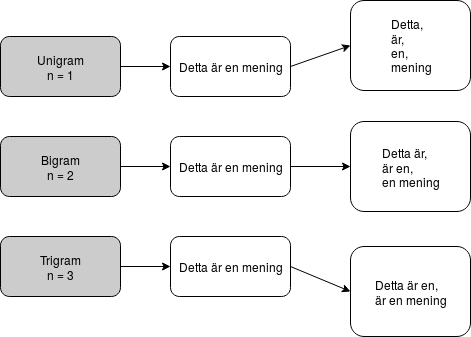
\includegraphics[width=9cm]{grams}
\centering
\caption{Illustration av n-grams på en mening.}
\label{fig:grams}
\end{figure}

Semantiska särdrag används mestadels för att ta ut  åsiktsord, sentimentord och negationer. Åsiktsord är ord eller meningar som kan innehålla någon typ av åsikt medan sentimentord är ord som innehåller något positivt eller negativt. Negationer är ett viktigt koncept eftersom en mening som innehåller någon typ av negation kan skifta om twitterinlägget är positivt eller negativt. Studien kommer använda sentimentord i lexikonimplementationen som diskuteras i avsnitt \ref{impl:lex} och negationer som även diskuterats i avsnitt \ref{exp:pre} kommer implementeras i avsnitt \ref{impl:pre}.

Syntaktiska särdrag används för att utforska påverkan av olika termer i SA och TSA, syntaktiska särdrag bryts ner till unigram, bigram, trigrams, n-gram, termfrekvens, omvänd dokumentfrekvens (IDF) och “Part of Speech” (POS). Där n-grams är ett samlingsord för uni-, bi- och trigram, i figur \ref{fig:grams} illustreras hur n-gram modellen fungerar på en enkel mening och hur meningens ord grupperas på olika sätta till ett ord eller fras. 

Termfrekvens används då längre twitterinlägg kan ha ett högre antal förekomster av ett ord än ett kortare twitterinlägg, vilket kan leda till att ord kan få större betydelse för klassificeringen. Genom användandet av termfrekvens delas antalet förekomster av ett ord i ett twitterinlägg med alla ord som finns i twitterinlägget undviks sådana problem \cite{scikit:001}. IDF \cite{idf:001} används i kombination med termfrekvens eftersom ordet “the” är så pass vanligt, kommer termfrekvens att lägga för stor vikt på ordet “the” som egentligen inte säger något om vilket sentiment twitterinlägget har. Så m.h.a IDF kommer ord som används sällan få större vikt och eventuell högre precision kan uppnås.


POS utförs genom att man räknar hur många substantiv, verb och adjektiv som existerar i ett twitterinlägg. POS kan t.ex användas för att ta reda på åsikter i ett twitterinlägg där antalet adjektiv kan relateras till vilken åsikt twitterinlägget har.

Studien kommer implementera unigram som ett bassärdrag för NB och SVM för att sedan utforska n-grams och termfrekvens för eventuell förhöjd prestanda vilket diskuteras i avsnitt \ref{impl}. POS kommer inte implementeras i studien då \cite{go2009twitter, feature:001} rapporterar försämrad precision. Däremot rapporteras i \cite{feature:002} små förbättringar vid användning av POS.

Stilistiska särdrag är särdrag som kommer från det informella skrivsättet som används på Twitter där t.ex emojis, förkortningar, slang och skiljetecken används. Enligt \cite{feature:002} kan emojis ha en stor betydelse för TSA. Men eftersom STS-datamängden har avlägsnat emojis, då “distant supervision” \cite{sts:001} har använts, kommer inte studiens modeller ta hänsyn till emojis. Därför har även emojis från SemEval-datamängden filtrerats bort i avsnitt \ref{exp:pre}. Studien kommer inte hantera slang eftersom inget större slanglexikon var öppet för användning. 
Förkortningar och skiljetecken kommer hanteras i denna studie och har diskuterats i avsnitt \ref{exp:pre} och implementeras i avsnitt \ref{impl:pre}.

Twitter-specifika särdrag är särdrag som är specifika för Twitters domän som t.ex “hashtags” och “mentions” vilka diskuterats i \ref{TSA} och \ref{exp:pre}.




\section{Algoritmer}
För att ge en bättre förståelse för hur NB, SVM och CNN kan appliceras på sentimentanalys, kommer detta avsnitt ge en överblick av hur algoritmerna går till väga för att klassificera text och hur de kan anpassas för att uppnå bra resultat vid sentimentanalys.

\subsection{Naive Bayes}
Det finns tre varianter utav NB nämligen Gaussian, Bernoulli och Multinomial. Gaussian används när attributen är kontinuerligt fördelade och då antas det att attributen förknippade med varje klass fördelas enligt Gaussian d.v.s normalfördelning \cite{nb:002}. Bernoulli användas när attributen är fördelade enligt multivariat Bernoulli \cite{nb:004} och Multinomial NB (MNB) används när attributen är multinomial fördelat. I \cite{nb:003} diskuteras det att MNB är väl lämpad för text klassificering vilket gör att studien kommer använda MNB.

I \ref{MLnb} beskrivs att Naive Bayes-algoritmen är baserad på Bayes theorem  \cite{wiki:009} vilket för TSA betyder att räkna ut sannolikheten att ett twitterinlägg $(B)$ är positivt eller negativt $(A)$ för en mängd $C$, bestående av ett antal $B$ med ett förbestämt $A$. Där $P(A | B)$ är en villkorlig sannolikhet för att $A$ inträffar givet att $B$ är sant, $P(B | A)$ är också en villkorlig sannolikhet för att $B$ inträffar givet att $A$ är sant. $P(A)$ och $P(B)$ är sannolikheten att observera $P(A)$ och $P(B)$ oberoende av varandra,

\begin{equation}\label{eq:bt}
P(A|B) = \frac{P(B|A) * P(A)}{P(B)}.
\end{equation}

För att ekvation \ref{eq:bt} skall vara “Naive”  antas att varje ord $b_w$ i $B$ är oberoende av varandra vilket betyder att vi inte längre klassificerar $B$ utan $b_w$, $P(B|A) = P(b_{w1}|A) * P(b_{w2}|A) * … * P(b_{wn}|A)$, där $n$ är antalet ord i $B$,

För att beräkna $P(b_w|A)$ används Dirichlet prior \cite{wiki:012, nb:007}, 
\begin{equation}\label{eq:slut}
P(b_w|A)= \frac{N_{b_w} + \alpha}{N_A + \alpha_n}.
\end{equation}
Där $N_{b_w}$ är hur många gånger $b_w$ förekommer i delmängden $C_A$, 
$N_A$ är summan av alla ord i $C_A$, $\alpha$ och $\alpha_n$ används för att utföra additiv utjämning \cite{wiki:013} där $\alpha = 1$ och $\alpha_n$ är summan av antal olika ord i $C$.

\begin{table}[H]
\centering
\caption{Exempeldatamängd med twitterinlägg som är märkta som positiva eller negativa.}
\label{tab:dataset}
    \begin{tabular}{ccc}
    \toprule
    \textbf{Twitterinlägg} & \textbf{Märkning} \\
    \midrule
    ser fram emot en dag i solen & Positiv \\
    jävla skitväder & Negativ \\
    vilken jävla kung du är linkan & Positv \\
    fyfan vilken dålig match & Negativ \\
    \bottomrule
\end{tabular}
\end{table}

I tabell \ref{tab:dataset} illustreras en datamängd $C$ med fyra twitterinlägg och deras märkning. Denna datamängd kan användas för att beräkna om twitterinlägget “solen skiner alltid i karlstad” $(B)$ är positivt eller negativt $(A)$ . Genom att räkna ut sannolikheten $P(Positiv|B)$ och $P(Negativ|B)$ kan märkning bestämmas, detta görs genom att jämföra vilken sannolikhet som blir störst och vi får följande ekvation,

\begin{equation}\label{eq:prodsum}
P(A|B) = \prod\limits_{i \epsilon B} \frac{P(i|A)}{P(B)},
\end{equation}

Och eftersom nämnaren är lika i bägge uträkningarna kommer enbart täljaren vara relevant vid beräkning.

För att räkna ut exempelvis $P(solen|Positiv)$ används ekvation \ref{eq:slut} där $N_{b_w} = 1$, $N_A= 13$, $\alpha_n = 17$ och $\alpha = 1$ vilket ger oss $P(solen|Positiv) =  \frac{1 + 1}{13 + 17} = 0,0667$. I tabell \ref{tab:ekv} illustreras alla ekvationer för att beräkna om “solen skiner alltid i karlstad” är positiv eller negativ. Ovanstående utförs på varje ord för både positiv och negativ vilket illustreras i tabell \ref{tab:ekv}.  Med hjälp av tabell \ref{tab:ekv} och ekvation \ref{eq:prodsum} beräknas, 

\begin{equation}
P(Positiv|\textrm{solen skiner alltid i karlstad}) = \frac{1.6428 * 10^-7}{P(B)},
\end{equation}
och
\begin{equation}
P(Negativ|\textrm{solen skiner alltid i karlstad}) =  \frac{1.5576 * 10^-7}{P(B)}.
\end{equation}

Jämförs dessa resultat kommer twitterinlägget klassificeras som positivt.

\begin{table}[H]
\centering
\caption{Beräkningar för om ett ord är positivt eller negativt.}
\label{tab:ekv}
    \begin{tabular}{ccc}
    \toprule
    \textbf{Ord} & \textbf{P(ord|Positiv)} & \textbf{P(ord|Negativ)} \\
    \midrule
    solen & $\frac{1 + 1}{13 + 17} $ & $\frac{0 + 1}{6 + 17} $\\
    skiner & $\frac{0 + 1}{13 + 17} $ & $\frac{0 + 1}{6 + 17}$ \\
    alltid & $\frac{0 + 1}{13 + 17}$ & $\frac{0 + 1}{6 + 17}$ \\
    i & $\frac{1 + 1}{13 + 17} $& $\frac{0 + 1}{6 + 17}$ \\
karlstad & $\frac{0 + 1}{13 + 17}$ & $\frac{0 + 1}{6 + 17}$ \\
    \bottomrule
\end{tabular}
\end{table}

\subsection{Support Vector Machine}
I avsnitt \ref{MLsvm} beskrevs SVM kortfattat, i detta avsnitt kommer SVM att beskrivas mer ingående. SVM-algoritmen skapar en modell utifrån en given mängd märkt träningsdata \cite{svm:002}. Modellen som skapas har sedan förmågan att kategorisera ny indata i en av de två kategorierna. Den skapade SVM-modellen representerar träningsdata som punkter i ett koordinatsystem. I koordinatsystemet kartläggs data så att de två kategorierna är tydligt separerade med ett så stort mellanrum som möjligt. När modellen kategoriserar ny indata kartläggs den datan till samma koordinatsystem, för att sedan kategoriseras utefter vilken sida av mellanrummet den hamnar på.

\begin{figure}[H]
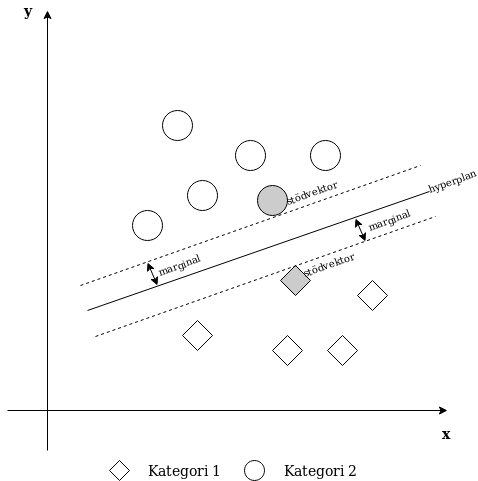
\includegraphics[width=9cm]{linearsvm_hpwithmargins}
\centering
\caption{Exempel på en linjär klassificerare där de två kateogrierna är linjärt separabla.}
\label{fig:svmmarg}
\end{figure}  

SVM separerar kategorierna genom att konstruera ett hyperplan \cite{svm:003}. Datapunkterna som hyperplanet positioneras utefter kallas stödvektorer. De är datapunkterna som ligger närmast hyperplanet från respektive kategori som ska klassificeras. I figur \ref{fig:svmmarg} representeras hyperplanet av linjen mellan kategorierna. Det kan finnas flera möjliga hyperplan som kan kategorisera datan. Idén bakom SVM är att hitta hyperplanet som bäst delar upp datamängden i två kategorier. Ju större marginal mellan kategorierna desto mindre känslig blir modellen för generaliseringsfel \cite{svm:002}. Därför anses hyperplanet som har störst marginal till stödvektorerna från respektive kategori ge en bra separation av data.

\begin{figure}[H]
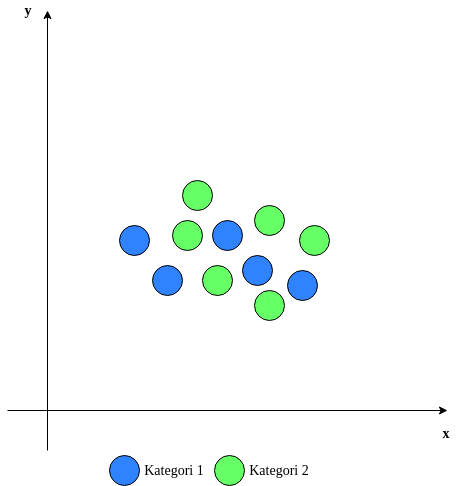
\includegraphics[width=9cm]{nonlinearsvm}
\centering
\caption{Exempel på en icke-linjär klassificeringsuppgift, där de två kategorierna inte är linjärt separabla.}
\label{fig:svmnonl}
\end{figure} 

Datapunkterna som SVM hanterar är vektorer av $p$ dimensioner, där varje dimension representerar ett särdrag. \cite{svm:002}. En linjär klassificerare definieras som en klassificerare där datapunkterna från de två kategorierna kan separeras med ett hyperplan av $p-1$ dimensioner. Klassificeringsuppgiften i figur \ref{fig:svmmarg} har två särdrag: x och y \cite{svm:005}. Datapunkterna i exemplet representeras således av en vektor av 2 dimensioner och de två kategorierna kan separeras med en linje. Exemplet i figur \ref{fig:svmmarg} representerar en linjär klassificerare, då de två kategorierna är linjärt separabla. 

Dock finns det klassificeringsproblem som inte går att separera linjärt, så kallade icke-linjära klassificeringsproblem. Figur \ref{fig:svmnonl} visar ett exempel på ett sådant problem. SVM kan även hantera sådana klassificeringsproblem \cite{svm:002}. I fall som dessa ritar SVM om datapunkterna till en högre dimension för att en separation ska bli möjlig, eftersom separationen förmodligen blir enklare i en högre dimension. Processen upprepas tills dess att ett hyperplan kan separera datan.  Metoden SVM använder för att utföra detta effektivt kallas “kernel trick” \cite{svm:004}. Detta illustreras i figur \ref{fig:svm3d}, där exemplet från figur \ref{fig:svmnonl} har ritats om i en högre dimension. Efter omritning till en högre dimension kan kategorierna separeras med ett plan. 

\begin{figure}[H]
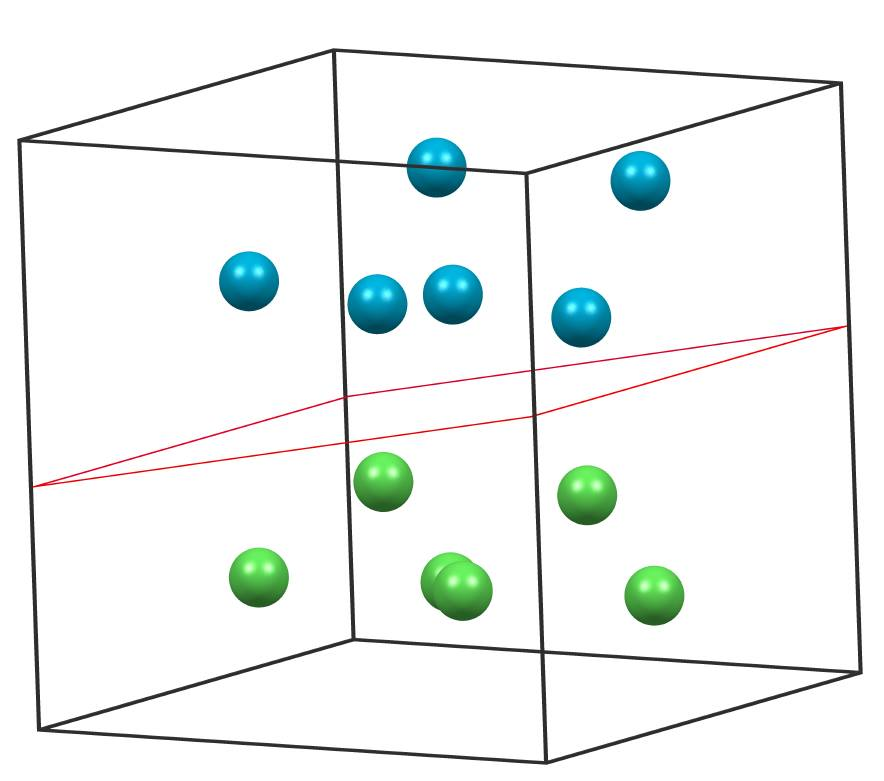
\includegraphics[width=9cm]{svm_3d}
\centering
\caption{Exemplet från figur \ref{fig:svmnonl} ritas om till en högre dimension.}
\label{fig:svm3d}
\end{figure} 

Om ett problem kräver en linjär eller en icke-linjär klassificerare beror på hur den data som ska klassificeras ser ut. Beteendet för SVM-algoritmen går att anpassa utefter den data som ska klassificeras genom att välja olika “kernel”-funktioner \cite{svm:006}. För textklassificering är det rekommenderat att använda en linjär “kernel”, vilket ger en linjär klassificerare. Anledningen till det är dels att de flesta textklassificeringsproblem är linjärt separerbara. Men det är även bra att använda en linjär “kernel” när antalet särdrag för klassificeringsproblemet är högt, vilket är fallet vid textklassificering. När antalet särdrag är högt är det ingen märkbar skillnad i prestanda mellan en linjär kontra icke-linjär “kernel”. Dessutom går en SVM-modell med en linjär “kernel” snabbare att träna än andra och det är färre parametrar som behöver justeras vid optimering av en modell. 
På grund av ovanstående anledningar har en linjär klassificerare valts att användas vid den här studien. 


\subsection{Convolutional Neural Network}
I avsnitt \ref{bak:cnn} beskrivs kortfattat vad CNN är och varför det på senare tid har börjat användas för maskininlärningsproblem som rör textbearbetning. I detta avsnitt kommer CNN att beskrivas på en mer teknisk nivå. De olika delarna som ett CNN består av kommer att presenteras, för att sedan beskriva hur ett CNN kan utföra textklassificering utifrån ett exempel. 

CNN är uppbyggt med flera lager \cite{cnn:005}. Det har ett lager för indata, ett för utdata och dessutom ett flertal dolda lager. De dolda lagrena består av konvulsionlager, “pooling”-lager, fullt ansluta lager och normaliseringslager. 

Konvulsionlager utgör den centrala delen av CNN \cite{cnn:005}. Ett konvulsionlager består av ett antal lärbara filter. I \cite{cnn:004} liknas en konvulsion med en funktion där ett fönster förflyttas över den data som ska analyseras, där datan är representerad som en matris. Fönstret som förflyttar sig över matrisen är det som kallas för filter. Vid varje förflyttning beräknas summan efter att filtrets värden har multiplicerat med respektive värde i matrisen. En hel konvulsion ges efter att fönstret har bearbetat hela matrisen.

“Pooling”-lager används vanligtvis efter konvultionslager \cite{cnn:004}. Det “pooling”-lager gör är att de tar ut en delmängd av den data de får in. Detta kan utföras med olika metoder, men en vanlig metod är att ta ut det största värdet från varje filter som bearbetas. Denna strategi kallas för “1-max pooling” \cite{cnn:002}. För klassificering krävs vanligtvis att de matriser som ges av filtrena har samma storlek \cite{cnn:004}. Genom användandet av “pooling” uppfylls det kravet, t.e.x om 100 filter används och “1-max pooling” appliceras på varje lager, kommer det alltid resultera i en vektor på 100 dimensioner. “Pooling” gör det alltså möjligt att skicka in data av varierande storlek och använda olika filterstorlekar, och alltid få ut den data som ska tolkas vid klassificeringen i samma storlek. En annan anledning till att “pooling”-lager används är att det minskar storleken på den data som ska analyseras samtidigt som den försöker behålla den mest relevanta informationen.

Efter att olika särdrag har tagits fram genom konvulsionlager och “pooling”-lager kopplas ett fullt ansluten lager in i slutet av nätverket \cite{cnn:008}. Det fullt anslutna lagret tar in mängden av särdrag från lagret innan och skickar ut en vektor av storleken $N$, där $N$ representerar antalet klasser vid klassificeringen. Värdena i denna vektor representerar sannolikheten för respektive klass. Det fullt anslutna lagret analyserar den data som skickas från lagret innan och gör en bedömning utefter vilken klass särdragen med störst sannolikhet representerar. 

Som nämndes i \ref{bak:cnn}, är CNN ursprungligen framtagen för problem som rör bearbetning av bilder. När bilder bearbetas av CNN representeras bildens pixlar i en matris, som filtrena sedan förflyttar sig över \cite{cnn:004}. Text som ska bearbetas av CNN behöver därför också representeras som en bild. I figur \ref{fig:cnntext} illustreras ett exempel av ett CNN för textklassificering. I exemplet ska ett twitterinlägg av längden $l$ klassificeras \cite{cnn:002}. Twitterinlägget som ska klassificeras har konverteras till en twitterinläggmatris. Varje ord i twitterinlägget utgör en rad i matrisen och representeras av en vektor i matrisen, där vektorernas dimension $d$ utgör matrisen bredd.  Matrisens storlek ges således av $l*d$.  Vektorerna som representerar olika ord är antingen ordinbäddningar \cite{wiki:016} eller “one-hot”-vektorer \cite{cnn:004}.  “One-hot”-vektorer är det som har använts för implementationen av CNN i denna studie och där indexeras varje ord i datamängden till ett vokabulär. Efter att twitterinlägget har konverterats till att representeras som en matris, går det att hantera inlägget som en bild och utföra konvulsioner på det genom olika filter \cite{cnn:002}. Eftersom varje rad representerar ett ord i twitterinlägget är det rimligt att använda filter som till bredden är lika stora som dimensionen på vektorerna. Höjden eller regionstorleken på filtren kan däremot varieras och det går att använda flertalet filter med olika regionstorlekar. Regionstorleken anpassas utefter hur många ord ett filter ska omfatta. 

\begin{figure}[H]
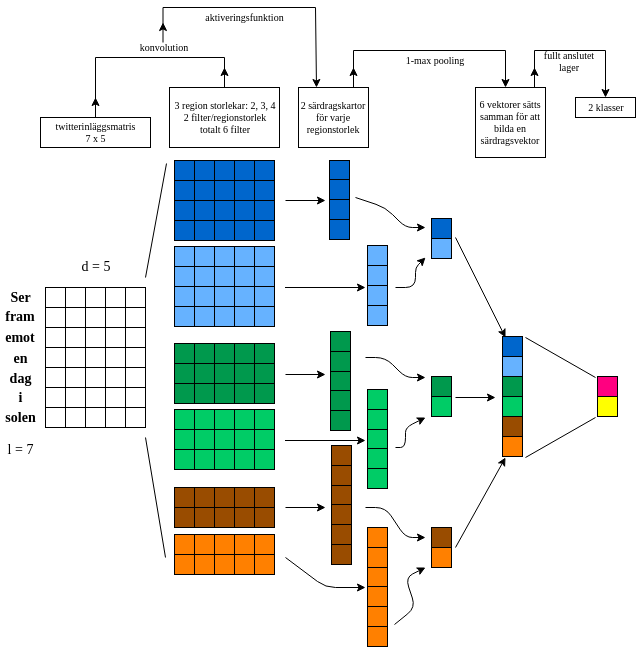
\includegraphics[width=12cm]{cnn_text}
\centering
\caption{Exempel på ett CNN som används för textklassificering. Figur inspirerad av \cite{cnn:002}.}
\label{fig:cnntext}
\end{figure}

I exemplet som illustreras i figur \ref{fig:cnntext} används tre olika regionstorlekar och två filter för varje regionstorlek, totalt används sex filter. Genom användandet av flertalet filter för respektive regionstorlek går det att få ut komplementerande särdrag från samma region \cite{cnn:002}. Från konvulsionerna som utförs på matrisen genereras särdragskartor. Den engelska termen är “feature maps”, men i denna studie har de valt att kallas för särdragskartor.  Storleken på varje särdragskarta som genereras kommer att variera beroende på twitterinläggets längd och regionstorleken på respektive filter. För att omvandla vektorerna till samma längd används en “pooling”-funktion på varje särdragskarta. Dessa vektorer sätts sedan samman till en ny vektor där twitterinläggets särdrag är representerade på en högre nivå. I slutet av nätverket har ett fullt anslutet lager kopplats in. Det fullt anslutna lagret tar slutligen in den sammankopplade vektorn och utför klassificeringen.



\section{Implementation}\label{impl}
Detta kapitel beskriver detaljer angående implementationen av vår studie och dess flöde som illustrerats i figur \ref{fig:overfig}. Kapitlet beskriver även teknikerna som används för att göra implementationen möjlig. Gemensamma tekniker som används i alla delar av implementation är programmeringsspråket Python3 \cite{impl:001} och Pandas \cite{impl:002}. Pandas är ett Python-paket som erbjuder snabba, flexibla datastrukturer som är utformade för att göra arbetet med relationell och märkt data smidigare. 
\subsection{Databearbetning}\label{impl:pre}
Som beskrivs i avsnitt \ref{exp:pre} är databearbetning ett viktigt steg inom SA och TSA. I detta avsnittet beskrivs implementationen av databearbetningen m.h.a delarna som illustreras i figur \ref{fig:dataset}.

För att avlägsna HTML-kod från twitterinlägg används BeautifulSoup \cite{impl:004}, som är ett Python-paket för att extrahera data från HTML-kod, om HTML-kod finns i twitterinlägg tas det således bort, se kodavsnitt \ref{pre:html}.
\begin{lstlisting}[style=mypython,caption={Test},label=pre:html]
def remove_html_encode(self):
       self.df["tweet"] = self.df["tweet"]./
       apply(lambda x: BeautifulSoup(x, 'lxml').get_text())
\end{lstlisting}

Omvandling från versaler till gemener utförs på varje twitterinlägg m.h.a den inbyggda Python-funktionen \pyth{str.lower()} som konverterar versaler till gemener, se kodavsnitt \ref{pre:lower}.
\begin{lstlisting}[style=mypython,caption={Test},label=pre:lower]
def to_lower(self):
      self.df["tweet"] = self.df["tweet"].str.lower()
\end{lstlisting}

Beskrivet i \ref{exp:pre} är expandering av sammandragsförkortningar ett viktigt moment för att kunna hantera negationer. Med  \pyth{cont_dic} kan vi hantera och expandera “can’t”, “won’t” och där ord slutar på “n’t”, se kodavsnitt \ref{pre:expand}
\begin{lstlisting}[style=mypython,caption={Test},label=pre:expand]
cont_dict = {'can\'t': 'cannot', 'won\'t': 'will not', 'n\'t': ' not'}
cont_re = re.compile('(%s)' % '|'.join(cont_dict.keys()))

def expand_cont(self, s, cont_dict=cont_dict):
       def replace(match):
                  return cont_dict[match.group(0)]
        return cont_re.sub(replace, s)

def expand_contractions(self):
       self.df["tweet"] = self.df["tweet"].apply(lambda x: self.expand_cont(x))
\end{lstlisting}

Avlägsna accenter utförs genom att använda \pyth{unicodedata.normalize()} \cite{impl:005} som använder “Normalization Form Compatibility Decomposition” (NFKD) parametern,  vilket betyder att \pyth{unicodedata.normalize()} byter ut en bokstav med accent mot sin ASCII-ekvivalenta bokstav. Resterande parametrar säger att om bokstaven redan är ASCII eller utf-8 ignoreras dessa bokstäver, se kodavsnitt \ref{pre:accent}.
\begin{lstlisting}[style=mypython,caption={Test},label=pre:accent]
def remove_accented_chars(self):
    self.df["tweet"] = self.df["tweet"].apply(lambda x:unicodedata./
    normalize('NFKD', x).encode('ascii', 'ignore')./
    decode('utf-8', 'ignore'))
\end{lstlisting}

I kodavsnitt \ref{pre:rem}  avlägsnas URL:er, “mentions”, “hashtags” , skiljetecken, siffror, emojis och repeterade mellanslag m.h.a fyra reguljära uttryck (RU) \cite{impl:003}. För att avlägsna URL:er används \pyth{'https?://[A-Za-z0-9./]+'} vilket betyder att om en URL är http eller https kommer denna avlägsnas.

“Mentions” avlägsnas med det RU \pyth{'@[A-Za-z0-9]+'}, d.v.s om en alfanumerisk sträng börjar med ‘@’ avlägsnas den alfanumeriska strängen.

Avlägsning av “hashtags”, skiljetecken, siffror och emojis görs med det RU \pyth{'[^a-zA-Z]'}, d.v.s en sträng måste börja på bokstäver mellan a-z, om inte tas dessa bort.

Och slutligen så avlägsnas repeterande mellanslag, vilket utförs med det RU \pyth{' +'}. Ifall det är två eller fler repeterande mellanslag tas dessa bort.

\begin{lstlisting}[style=mypython,caption={Test},label=pre:rem]
def remove_links(self):
       self.df.loc[:, "tweet"] = self.df.loc[:, "tweet"].\
       replace(r'https?://[A-Za-z0-9./]+', '', regex=True)

def remove_twitter_mention(self):
       self.df.loc[:, "tweet"] = self.df.loc[:, "tweet"].\
       replace(r'@[A-Za-z0-9]+', '', regex=True)

def remove_hashtag(self):
       self.df.loc[:, "tweet"] = self.df.loc[:, "tweet"].\
       replace('[^a-zA-Z]', ' ', regex=True)

def remove_extra_whitepsace(self):
      self.df.loc[:, "tweet"] = self.df.loc[:, "tweet"].\
       replace(' +', ' ', regex=True)
\end{lstlisting}

För att utföra ordstamsigenkänning och avlägsning av stoppord måste varje twitterinlägg först tokeniseras, vilket betyder att varje ord i ett twitterinlägg blir ett eget element i en lista. Tokeniseringen utförs m.h.a funktionen \pyth{word_tokenize()} \cite{impl:006} från Natural Language Toolkit (NLTK), se kodavsnitt \ref{pre:token}.
\begin{lstlisting}[style=mypython,caption={Test},label=pre:token]
def tokenize(self):
      self.df["tweet"] = self.df["tweet"].apply(word_tokenize)
\end{lstlisting}

I kodavsnitt \ref{pre:stem} utförs ordstamsigenkänning m.h.a \pyth{SnowballStemmer('english').stem()} \cite{impl:008} från NLTK som försöker hitta varje ords ordstam vilket diskuteras i avsnitt \ref{exp:pre}.
\begin{lstlisting}[style=mypython,caption={Test},label=pre:stem]
def word_stemming(self):
       self.df["tweet"] = self.df["tweet"]./
       apply(lambda x: [SnowballStemmer('english').stem(y) for y in x])
\end{lstlisting}

Avlägsning av stoppord utförs m.h.a \pyth{stopwords.word('english')} \cite{impl:007} från NLTK som är en lista av engelska stoppord. \pyth{Remove_stopwords()} kontrollerar om något ord i twitterinlägget finns med i listan, om det gör det tas det bort, se kodavsnitt \ref{pre:stop}.
\begin{lstlisting}[style=mypython,caption={Test},label=pre:stop]
stop = stopwords.words('english')
def remove_stopwords(self):
       self.df["tweet"] = self.df["tweet"]./
       apply(lambda x: [word for word in x if word not in stop])
\end{lstlisting}
\subsection{Lexikon}\label{impl:lex}
I detta avsnitt diskuteras hur den lexikonbaserade modellen implementeras som blir ett basfall för STS- och SemEval-datamängden. Tekniker som använts för implementationen är WordNet \cite{lex:001} och SentiWordNet \cite{lex:002} från python-paketet NLTK.
WordNet är en lexikal databas på engelska som hittar konceptuella relationer mellan ord där substantiv, verb, adjektiv och adverb grupperas till mängder av kognitiva synonymer. SentiWordNet använder sedan de kognitiva synonymerna för att klassificera om de är positiva eller negativa.

I kodavsnitt \ref{lex:kod} illustreras implementationen av den lexikonbaserade modellen, som tar ett twitterinlägg som parameter. Twitterinlägget delas sedan ner till en mängd ord med respektive POS-tag. Därefter utförs tre kontroller på respektive ord. Den första kontrollen kontrollerar om ordet är ett substantiv, adjektiv eller ett adverb. Sedan kontrolleras om ordet har en grundform och slutligen kontrolleras om ordet är en synonym. Om ordet inte klarar de tre kontrollerna hoppar vi över ordet, eftersom ordet inte kan klassificeras. Ifall ordet går igenom kontrollerna tas ordets klassificering fram och adderas till en variabel $sentiment$. När alla mängdens ord antingen har klassificerats eller hoppats över används $sentiment$ för att klassificera om twitterinlägget är positivt eller negativt, d.v.s om $sentiment >= 0$ är inlägget positivt annars negativt.

\begin{lstlisting}[style=mypython,caption={Test},label=lex:kod]
def swn_classifier(tweet):
    sentiment = 0.0
    tokens_count = 0

    sentinized_tweet = sent_tokenize(tweet)

    for sentence in sentinized_tweet:
        # Part of Speach tag
        tagged_tweet = pos_tag(word_tokenize(sentence))

        for word, tag in tagged_tweet:
            wn_tag = convert_tag(tag)
            if wn_tag not in (wn.NOUN, wn.ADJ, wn.ADV):
                continue

            lemma = lemmatizer.lemmatize(word, pos=wn_tag)
            if not lemma:
                continue

            synset = wn.synsets(lemma, pos=wn_tag)
            if not synset:
                continue

            synset = synset[0]
            swn_synset = swn.senti_synset(synset.name())

            sentiment += swn_synset.pos_score() - swn_synset.neg_score()
            tokens_count += 1

    if not tokens_count:
        return 0

    if sentiment >= 0:
        return 1

    return 0
\end{lstlisting}
Kodavsnitt \ref{lex:kod} körs på både STS- och SemEval-datamängden där resultatet presenteras i avsnitt \ref{res}.

\subsection{Naive Bayes}\label{impl:nb}
I detta avsnitt diskuteras hur Naive bayes-algoritmen implementerats och hur vi anpassat algoritmens parametrar för att uppnå ett eventuellt förbättrad precision. För implementation av NB har SciKit-learn (sk-learn) \cite{scikit:002} använts, som är ett Python-paket för maskininlärning.

För att implementera och träna Naive bayes-algoritmen måste först datamängden delas in i en tränings- och en testmängd. Delningen utförs för att möjliggöra utvärdering av algoritmens precision, vilket testmängden används för. Delningen utförs m.h.a sk-learn funktionen \pyth{train_test_split()} \cite{scikit:003} där datamängden delas till 20\% testmängd och 80\% träningsmängd, se kodavsnitt \ref{impl:datasplit}.
\begin{lstlisting}[style=mypython,caption={Test},label=impl:datasplit]
X_train, X_test, y_train, y_test = train_test_split(df.tweet,
            df.lable, test_size=0.2, random_state=0)
\end{lstlisting}

I kodavsnitt \ref{nb:base} implementeras algoritmen \pyth{MultinomialNB()} med standardparametrar \cite{scikit:004} och unigram som särdrag vilket är standard parameter för \pyth{CountVectorizer()} \cite{scikit:005}. Träningen av algoritmen utförs med \pyth{fit(X_train, y_train)} funktionen som tar träningsmängden som indata. Precisionen tas fram genom att först klassificera vår testmängd på den tränade algoritmen m.h.a \pyth{predict(X_test)} för att sedan använda \pyth{metrics.classification_report()} som presenterar värden som diskuterats i avsnitt \ref{TSAev}.
\begin{lstlisting}[style=mypython,caption={Test},label=nb:base]
nb_unigram_clf = Pipeline([('vect', CountVectorizer()), ('clf', MultinomialNB())])
nb_unigram_clf.fit(X_train, y_train)
predicted = nb_unigram_clf.predict(X_test)
print(metrics.classification_report(y_test, predicted, target_names=target_names))
\end{lstlisting}
Kodavsnitt \ref{nb:base} körs på både STS- och SemEval-datamängden där resultatet presenteras i avsnitt \ref{res}.

I kodavsnitt \ref{nb:grid} används \pyth{GridSearchCV()} \cite{scikit:006} vilket är en sk-learn funktion för att utföra parametersökning för algoritmer och särdragsfunktioner så att optimala parametrar kan hittas. För \pyth{CountVectorizer()} är vi intresserade av $max_df$ och $ngram_range$. $Max_df$ tar emot ett flyttal mellan intervallet $[0.0, 1.0]$ som under uppbyggnaden av vokabuläret ignorerar ord som har en twitterinläggsfrekvens högre än det angivna flyttalet. $Ngram_range$ används för att testa vilken typ av ngram som skall användas, t.e.x (1, 1) betyder unigram och (1, 2) betyder att både uni- och bigrams används.

För \pyth{TfidfTransformer()} är vi intresserade av \pyth{use_idf} och \pyth{norm}. \pyth{Use_idf} används för att specificera om IDF skall användas eller ej. \pyth{Norm} specificerar vilken typ av normaliserings funktion som används för att normalisera vår ord vektor.\pyth{SelectKBest()} \cite{scikit:007} tar två parametrar, \pyth{score_func} och $k$. För \pyth{score_func} är vi bara intresserade av “chi-squared test” (chi2) och $k$ är ett heltal för hur många av dem  bästa särdrag som tas ut från \pyth{score_func}. Eftersom MNB är en så pass enkel klassificeringsalgoritm finns det inga parametrar att justera.

\begin{lstlisting}[style=mypython,caption={Test},label=nb:grid]
pipeline = Pipeline([
    ('vect', CountVectorizer()),
    ('tfidf', TfidfTransformer()),
    ('kbest', SelectKBest(chi2)),
    ('clf', MultinomialNB()),
])
parameters = {
    'vect__max_df': (0.5, 0.75, 1.0),
    'vect__ngram_range': ((1, 1), (1, 2), (1, 3)),  # uni-, bi-, trigram
    'tfidf__use_idf': (True, False),
    'tfidf__norm': (None, 'l1', 'l2'),
    'kbest__k': (x),
}

grid_search = GridSearchCV(pipeline, parameters, n_jobs=-1, verbose=1)
\end{lstlisting}

Kodavsnitt \ref{nb:grid} kör både STS- och SemEval-datamängderna, där \pyth{'kbest__k': (x)} är den parameter som differentierar mellan datamängderna. I tabell \ref{tab:kbest} illustreras antal särdrag som vardera datamängd har och vilket intervall $x$ sätts till för vardera datamäng. Resultatet av körningarna presenteras i avsnitt \ref{res}

\begin{table}
\centering
\caption{Illustrerar antal särdrag för STS- och SemEval-datamängderna och vilket intervall vi använder för parametersökning.}
\label{tab:kbest}
    \begin{tabular}{ccc}
    \toprule
     & \textbf{Antal särdrag} & \textbf{x} \\
    \midrule
    \textbf{SemEval} & 10272 & (3000, 6000, 8000, 'all') \\ 
    \textbf{STS} & 200000 & (30000, 50000, 100000, 130000, 'all') \\
    \bottomrule
\end{tabular}
\end{table}




\subsection{Support Vector Machine}\label{impl:svm}
I detta avsnitt diskuteras hur SVM-algoritmen implementerats och hur vi anpassat algoritmens parametrar för att uppnå ett eventuellt förbättrad precision. SVM har också implementeras m.h.a sk-learn.

I avsnitt \ref{impl:nb} diskuteras att en datamängd först måste delas in i en test- och träningsmängd, vilket även är fallet för SVM. Uppdelningen sker på samma sätt som illustreras i kodavsnitt \ref{impl:datasplit}. 

I kodavsnitt \ref{svm:base} implementeras algoritmen \pyth{SGDClassifier()} med standard parametrar \cite{scikit:009}. \pyth{SGDClassifier()} är en linjär klassificerare baserat på en SVM med “stochastic gradient descent” (SGD) träning. Valet att använda \pyth{SGDClassifier()} istället för en ren linjär SVM är p.g.a att \pyth{SGDClassifier()} är bättre anpassad för stora datamängder \cite{scikit:008}, vilket är fallet för studien då STS-datamängden används. Som särdrag används unigram vilket är standardparametern för \pyth{CountVectorizer()}.

Träningen av algoritmen utförs med funktionen \pyth{fit(X_train, y_train)}, som tar träningsmängden som indata. Precisionen tas fram genom att klassificera testmängden på den tränade algoritmen m.h.a \pyth{predict(X_test)}. Sedan används \pyth{metrics.classification_report()} för att presentera utvärderingsvärdena som diskuteras i avsnitt \ref{TSAev}.
\begin{lstlisting}[style=mypython,caption={Test},label=svm:base]
svm_unigram_clf = Pipeline([
	('vect', CountVectorizer()), 
	('clf', SGDClassifier())
])
svm_unigram_clf.fit(X_train, y_train)
predicted = svm_unigram_clf.predict(X_test)
print(metrics.classification_report(y_test, predicted, target_names=target_names))
\end{lstlisting}

För parametersökningen som illustreras i kodavsnitt \ref{svm:grid} används \pyth{GridSearchCV()}. Vi är intresserade utav samma parametrar för \pyth{CountVectorizer(), TfidfTransformer()} och \pyth{SelectKBest()} som diskuteras i avsnitt \ref{impl:nb}. För klassificeringsalgoritmen \pyth{SGDClassifier()} är följande parametrar av intresse: \pyth{max_iter}, \pyth{penalty} och \pyth{alpha}. \pyth{Max_iter} är hur många gånger algoritmen går igenom datamängden, \pyth{penalty} specificerar vilken typ av normaliseringsfunktion som används för att undvika överanpassning \cite{svm:007}. Överanpassning är ett fenomen där klassificeringsalgoritmen under träning lär sig detaljerna i datamängden vilket kommer skada precisionen när ny data klassificeras.
\pyth{Alpha} används för att specificera vilken initial inlärningsfrekvens algoritmen använder.

\begin{lstlisting}[style=mypython,caption={Test},label=svm:grid]
pipeline = Pipeline([
    ('vect', CountVectorizer()),
    ('tfidf', TfidfTransformer()),
    ('kbest', SelectKBest(chi2)),
    ('clf', SGDClassifier()),
])
parameters = {
    'vect__max_df': (0.5, 0.75, 1.0),
    'vect__ngram_range': ((1, 1), (1, 2), (1, 3)),
    'tfidf__use_idf': (True, False),
    'tfidf__norm': (None, 'l1', 'l2'),
    'kbest__k': (x),
    'clf__alpha': (1e-4, 1e-3, 1e-2, 1e-1, 1e0, 1e1),
    'clf__max_iter': (500, 1000, 1500),
    'clf__penalty': ('l2', 'l1', 'elasticnet'),
}

grid_search = GridSearchCV(pipeline, parameters, n_jobs=-1, verbose=1)
\end{lstlisting}

Resultatet av parametersökningen presenteras i avsnitt \ref{res}.
\subsection{Convolutional neural network}
För implementationen av CNN har en referensimplementation använts, som har anpassats för att analysera twitterinlägg. Referensimplementationen har implementerades med Keras \cite{impcnn:004}. Keras är ett högnivåbibliotek för djup inlärning skrivet i Python, som utvecklades för att göra det snabbt och enkelt att experimentera med neuronnät. Det kan bland annat köras ovanpå TensorFlow \cite{impcnn:005}, som är ett “open-source”-bibliotek för numerisk beräkning med starkt stöd för maskininlärning och djup inlärning. 

I \cite{impcnn:003} presenteras referensimplementationen. Referensimplementationen är en förenklad implementation av Britz implementation \cite{impcnn:002}, som har implementerats med TensorFlow. Britz förklarar och presenterar sin implementation steg för steg i \cite{impcnn:001}. Implementationen är baserad på Kims modell \cite{cnn:003}  som nämndes i avsnitt \ref{bak:cnn}. Men Britz har förenklat modellen något, exempelvis används inte tränande ordinbäddningar utan istället använts “one-hot”-vektorer för att representera ord.

Parametrarna som används i referensimplementationen skiljer sig dock från standardparametrarna som används i Britz implementation. För implementationen i den här studien har standardparametrarna från Britz implementation använts istället för de som används i referensimplementationen. I kodavsnitt \ref{cnn:par} presenteras parametrar som har använts för denna studie. Parametrarna används bland annat för att bestämma storleken på twitterinläggsmatrisen, storleken på de filter som ska användas och antalet filter för varje regionstorlek. Dessa beskrevs tidigare i avsnitt \ref{exp:cnn}. Höjden och bredden på twitterinläggsmatrisen representeras i kodavsnittet av \pyth{sequence_length = x.shape[1]} och \pyth{embedding_dim = 128}.

Parametern \pyth{drop = 0.5} används i “Dropout”-lagret för att bestämma hur stor del av neuronnätets enheter, som slumpmässigt ska kopplas bort vid varje uppdatering under träningen \cite{impcnn:006}. “Dropout”-lagret används för att undvika överanpassning. Vid träningen av en modell anges hur många gånger modellen ska tränas på en given datamängd \cite{impcnn:007}. Detta kallas för epoker och i koden har det angetts genom parametern \pyth{ephocs = 100}. Parametern \pyth{batch_size = 64} anger hur många exempel från träningsdatamängden som ska neuronätet ska tränas på åt gången \cite{impcnn:007}.

\begin{lstlisting}[style=mypython,caption={Test},label=cnn:par]
sequence_length = x.shape[1]
vocabulary_size = len(vocabulary_inv)
embedding_dim = 128
filter_sizes = [3, 4, 5]
num_filters = 128
drop = 0.5
epochs = 100
batch_size = 64
\end{lstlisting}

Databearbetningen som används i referensimplementationen har ändrats till den som beskrivs i avsnitt \ref{exp:pre}. Detta för att modellerna ska kunna utvärderas efter samma förutsättningar. Uppdelningen av datamängderna har utförts på samma sätt som diskuteras i \ref{impl:nb}

Koden i kodavsnitt \ref{cnn:input} används för att skapa lagret som hanterar data som skickas in och twitterinläggsmatrisen som ska användas för att analysera twitterinläggen.

\begin{lstlisting}[style=mypython,caption={Test},label=cnn:input]
inputs = Input(shape=(sequence_length,), dtype='int32')

embedding = Embedding(input_dim=vocabulary_size, output_dim=embedding_dim,
			input_length=sequence_length)(inputs)
			
reshape = Reshape((sequence_length, embedding_dim, 1))(embedding)
\end{lstlisting}

I kodavsnitt \ref{cnn:conv} skapas tre konvulsionlager. Arkitekturen är densamma som illustreras i \ref{fig:cnntext}, men istället för att det används enbart två filter för varje filterstorlek används istället \pyth{num_filters = 128} filter för respektive filterstorlek i implementation.

\begin{lstlisting}[style=mypython,caption={Test},label=cnn:conv]
conv_0 = Conv2D(num_filters, kernel_size=(filter_sizes[0], embedding_dim), 
    padding='valid', kernel_initializer='normal', activation='relu')(reshape)
	
conv_1 = Conv2D(num_filters, kernel_size=(filter_sizes[1], embedding_dim), 
    padding='valid', kernel_initializer='normal', activation='relu')(reshape)
	
conv_2 = Conv2D(num_filters, kernel_size=(filter_sizes[2], embedding_dim), 
    padding='valid', kernel_initializer='normal', activation='relu')(reshape)
\end{lstlisting}

Sedan appliceras “pooling”-lager på respektive konvolutionslager, se kodavsnitt \ref{cnn:pool}. 

\begin{lstlisting}[style=mypython,caption={Test},label=cnn:pool]
maxpool_0 = MaxPool2D(pool_size=(sequence_length - filter_sizes[0] + 1, 1),
    strides=(1,1), padding='valid')(conv_0)
	
maxpool_1 = MaxPool2D(pool_size=(sequence_length - filter_sizes[1] + 1, 1), 
    strides=(1,1), padding='valid')(conv_1)
	
maxpool_2 = MaxPool2D(pool_size=(sequence_length - filter_sizes[2] + 1, 1), 
    strides=(1,1), padding='valid')(conv_2)
\end{lstlisting}

Det som skickas ut från “pooling”-lagrena sätts samman till en ny särdragsvektor genom \pyth{Concatenate(axis=1)([maxpool_0, maxpool_1, maxpool_2])}. Ett fullt anslutet lager skapas med \pyth{Dense()} \cite{impcnn:006}, som tar in den särdragsvektorn och utför klassificeringen av twitterinlägg. Innan klassificeringen, appliceras först \pyth{Flatten()} \cite{impcnn:006} och sedan \pyth{Dropout()} \cite{impcnn:006} på särdragsvektorn, se kodavsnitt \ref{cnn:output}. \pyth{Flatten()} används för att ändra representationen av särdragsvektorn och \pyth{Dropout()} används för att undvika överanpassning. 

\begin{lstlisting}[style=mypython,caption={Test},label=cnn:output]
concatenated_tensor = Concatenate(axis=1)([maxpool_0, maxpool_1, maxpool_2])
flatten = Flatten()(concatenated_tensor)
dropout = Dropout(drop)(flatten)
output = Dense(units=2, activation='softmax')(dropout)
\end{lstlisting}

Modellen skapas med klassen \pyth{Model()} \cite{impcnn:008}. För att konfigurera modellen inför träning används metoden \pyth{compile()} \cite{impcnn:008} och för träna modellen används metoden \pyth{fit()} \cite{impcnn:008}. Skapandet och träningen av modelllen i referensimplementationen illustreras i kodavsnitt \ref{cnn:model}

\begin{lstlisting}[style=mypython,caption={Test},label=cnn:model]
model = Model(inputs=inputs, outputs=output)

checkpoint = ModelCheckpoint('weights.{epoch:03d}-{val_acc:.4f}.hdf5', 
    monitor='val_acc', verbose=1, save_best_only=True, mode='auto')

adam = Adam(lr=1e-4, beta_1=0.9, beta_2=0.999, epsilon=1e-08, decay=0.0)

model.compile(optimizer=adam, loss='binary_crossentropy', metrics=['accuracy'])

model.fit(X_train, y_train, batch_size=batch_size, epochs=epochs, verbose=1, 
    callbacks=[checkpoint], validation_data=(X_test, y_test))
\end{lstlisting}

Zhang och Wallace förklarar i \cite{cnn:002} att en negativ sida av CNN är att utvecklare måste ha kunskap nog att specificera den exakta arkitekturen av modellen och dessutom ställa in alla medföljande parametrar.  Parametrarna är så pass många till antalet att det kan vara överväldigande för en utvecklare som nyligen introducerats för tekniken. Att undersöka olika typer av konfigurationer av dessa parametrar är dessutom väldigt kostsamt. Dels för att det tar lång tid att träna den här typen av modeller, men även pga att antalet möjliga inställningar av dessa parametrar är så pass många. Av de anledningarna har ingen parametersökning utförts på CNN. Därför har enbart en CNN-modell tagits fram för detta experiment, med standardparametrarna från Britz implementation \cite{impcnn:002}.






\subsection{Webbgränssnitt}
Som ett alternativ till studiens syfte hade uppdragsgivaren ett önskemål av en webbsida där en dynamisk sökning kunde utföras på en Twitter-användare, för att sedan presentera hur klassiciferingsmodellerna klassificerar Twitter-användarens twitterinlägg.
Tekniker som valts för webbsidans gränssnitt är Bootstrap \cite{gui:001} och för webbsidans bakände används Flask \cite{gui:002} och SQLite3 \cite{gui:003}.
Bootstrap är ett “open source” verktyg framtaget av Twitter för att bygga responsiva, mobila projekt på webben med HyperText Markup Language (HTML), Cascading Style Sheets (CSS) och Javascript (JS). Flask är ett mikro webbramverk som används för att prata med bakände funktioner och rendera webbsidans gränssnitt. För att lagra resultaten från sökningen har SQLite3 används som databashanterare.

I figur \ref{fig:gui_form} illustreras implementationen av webbgränssnittet där användare kan söka på en Twitter-användare och hur många twitterinlägg som ska klassificeras.

\begin{figure}[H]
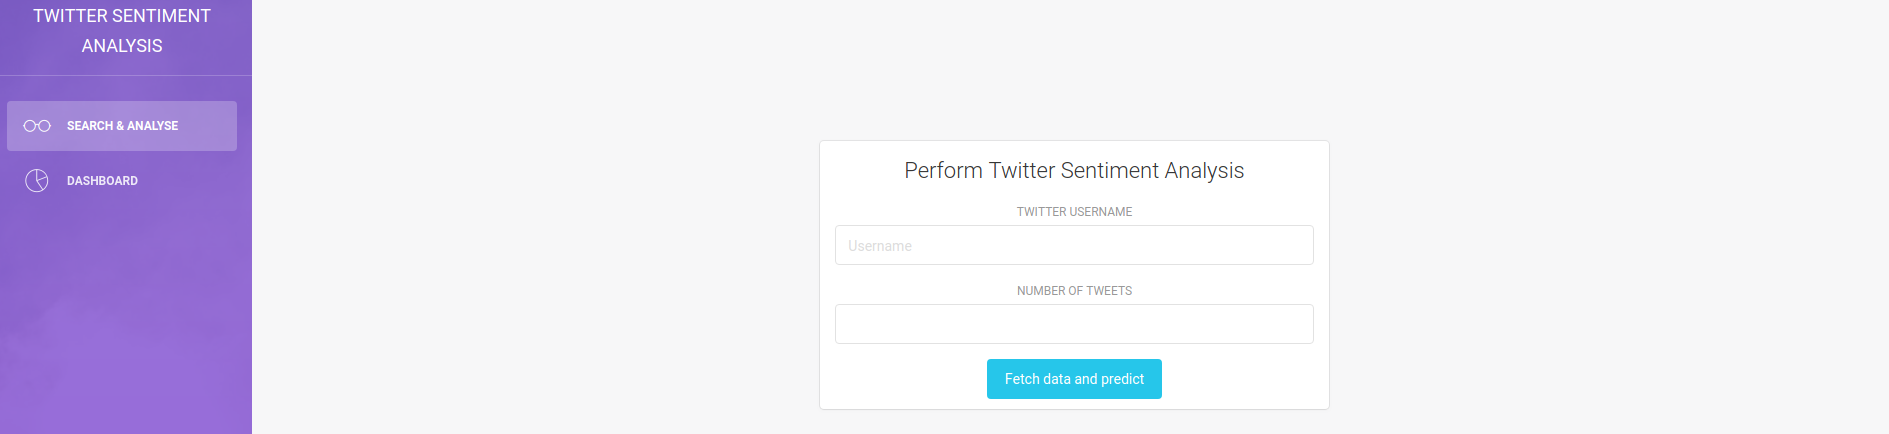
\includegraphics[width=12cm]{GUI_form}
\centering
\caption{Illustrerar webbgränssnittets sökformulär.}
\label{fig:gui_form}
\end{figure}

I figur \ref{fig:gui_search_g} illustreras en pajgraf för vardera klassificeringsmodell som visar hur många av de inhämtade twitterinläggen från Twitter-användaren “realDonaldTrump” som är positiva eller negativa.

\begin{figure}[H]
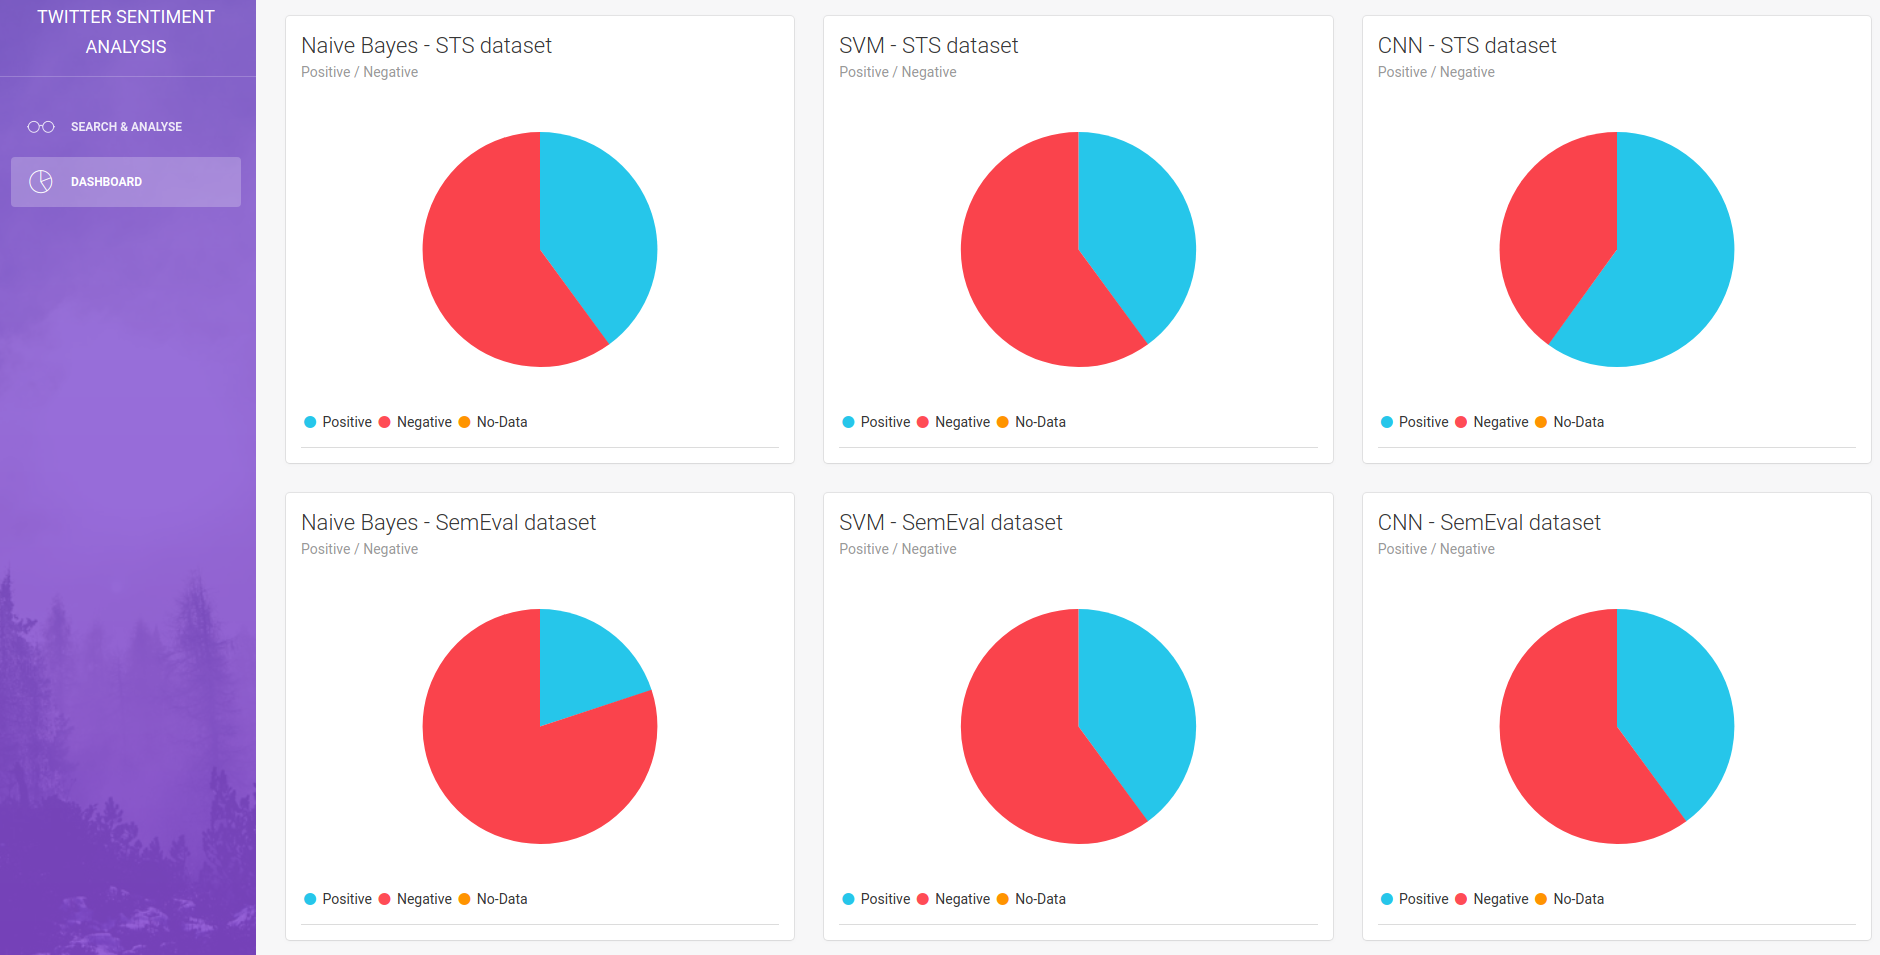
\includegraphics[width=12cm]{GUI_search_graph}
\centering
\caption{Illustrerar hur klassificeringsmodellerna har klassificerat 10 stycken twitterinlägg från användaren “realDonaldTrump” som är inhämtade 2018-04-16 11:40.}
\label{fig:gui_search_g}
\end{figure}

Figur \ref{fig:gui_search_t} illustrerar de inhämtade twitterinläggen från användaren “realDonaldTrump” i en tabell där användare kan analysera hur varje klassificeringsmodell har klassificerat varje twitterinlägg.

\begin{figure}[H]
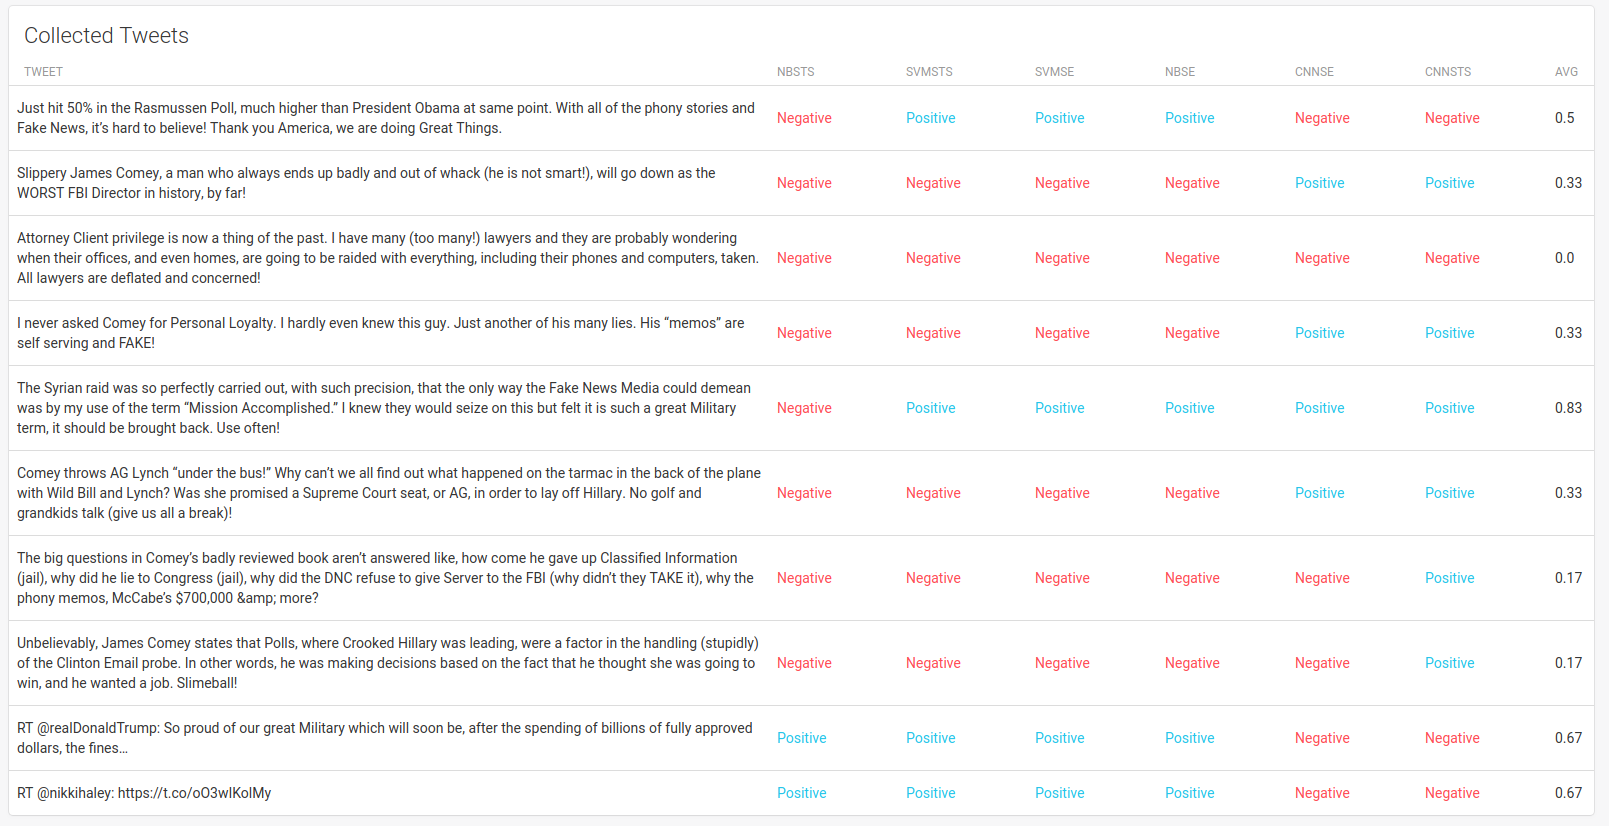
\includegraphics[width=12cm]{GUI_search_table}
\centering
\caption{Illustrerar hur klassificeringsmodellerna har klassificerat varje tweet.}
\label{fig:gui_search_t}
\end{figure}
\section{Sammanfattning}
I detta kapitel har tillvägagångssättet för studiens experiment diskuterats. En teknisk fördjupning har presenterats för databearbetning, särdragsurval och de tre algoritmerna, NB, SVM och CNN. Utöver detta presenteras även implementeringen av databearbetning, särdragsurval och de tre algoritmerna, där även ett webbgränssnitt har tagits fram på uppdragsgivarens önskemål.

\chapter{Resultat} \label{res}
\section{Intro}
\section{Resultatet mellan modellerna}
\subsection{Dataset 1 -> jämför resultat mellan modellerna}
\subsection{Dataset 2 -> jämför resultat mellan modellerna}
\newpage
\section{Implementations mässigt vilken modell är lättast?}
\section{implementations jämförelse (resultat VS förväntat)}
\section{Summering}

\chapter{Slutsats}
\section{Sammanfattning}
\section{Problem}
\section{Begränsningar}
\newpage
\section{Vidare utveckling}
\section{Slutord}



\bibliographystyle{unsrtnat} 
\bibliography{../refs/thesisref}


\restoregeometry%

\end{document}
\endinput
%%
%% End of file `kaumasterstemplate.tex'.
